%%\title{Physical Elements and Markers}
%  Changed by: Chris ISELIN, 24-Jan-1997 
%  Changed by: Hans Grote, 25-Sep-2002

\chapter{Elements and Markers}

%\begin{itemize}
%	\item \href{elm_format.html}{Element Input Format}
%	\item \href{aperture.html}{Aperture, Geometric}
%	\item \href{marker.html}{MARKER: Marker Definition}
%	\item \href{drift.html}{DRIFT: Drift Space}
%	\item \href{bend.html}{Bending Magnet}
%\begin{itemize}
%	\item \href{bend.html#rbend}{RBEND: Rectangular Bending Magnet}
%	\item \href{bend.html#sbend}{SBEND: Sector Bending Magnet}
%	\item \href{dipedge.html}{Dipedge Element}
%\end{itemize}
%	\item \href{quadrupole.html}{QUADRUPOLE}
%	\item \href{sextupole.html}{SEXTUPOLE}
%	\item \href{octupole.html}{OCTUPOLE}
%	\item \href{multipole.html}{MULTIPOLE}
%	\item \href{solenoid.html}{SOLENOID}
%	\item \href{nllens.html}{Non-linear lenses: elliptic potential}
%	\item \href{kickers.html}{Closed Orbit Corrector}
%\begin{itemize}
%	\item \href{kickers.html#hkick}{HKICKER: Horizontal Orbit Corrector}
%	\item \href{kickers.html#vkick}{VKICKER: Vertical Orbit Corrector}
%	\item \href{kickers.html#kick}{KICKER: Combined Orbit Corrector}
%\end{itemize}
%	\item \href{tkickers.html}{Transverse Kicker}
%	\item \href{cavity.html}{RFCAVITY}
%	\item \href{rfmultipole.html}{RFMULTIPOLE}
%	\item \href{crabcavity.html}{CRABCAVITY}
%	\item \href{separator.html}{ELSEPARATOR: Electrostatic Separator}
%	\item \href{monitors.html}{Beam Position Monitor}
%\begin{itemize}
%	\item \href{monitors.html#hmon}{HMONITOR: Horizontal Monitor}
%	\item \href{monitors.html#vmon}{VMONITOR: Vertical Monitor}
%	\item \href{monitors.html#mon}{MONITOR: Combined Monitor}
%	\item \href{monitors.html#inst}{INSTRUMENT: Other Beam Instrumentation}
%\end{itemize}
%	\item \href{collimator.html}{Collimators}
%\begin{itemize}
%	\item \href{collimator.html#rcol}{RCOLLIMATOR:Rectangular Collimator}
%	\item \href{collimator.html#ecol}{ECOLLIMATOR:Elliptic Collimator}
%\end{itemize}
%	\item \href{rotation.html}{Coordinate Transformations}
%\begin{itemize}
%	\item \href{rotation.html#yrotation}{YROTATION: Rotation About the Vertical Axis}
%	\item \href{rotation.html#srotation}{SROTATION: Rotation Around the Longitudinal Axis}
%\end{itemize}
%	\item \href{beambeam.html}{BEAMBEAM: Beam-Beam Interaction}
%	\item \href{matrix.html}{MATRIX: Arbitrary Element}
%	\item \href{elm_edit.html}{Editing Element Definitions}
%	\item \href{elm_class.html}{Element Class}
%\end{itemize}

%\href{http://www.cern.ch/Hans.Grote/hansg_sign.html}{hansg}, January 24, 1997 

% add other files to the end of this file

\section{Definitions}

%%%\title{Element Input Format}
%  Changed by: Chris ISELIN, 24-Jan-1997 

%  Changed by: Hans Grote, 22-Jan-2003 

%%\usepackage{hyperref}
% commands generated by html2latex


%%\begin{document}
%%\begin{center}
 %%EUROPEAN ORGANIZATION FOR NUCLEAR RESEARCH 
%%\includegraphics{http://cern.ch/madx/icons/mx7_25.gif}

\subsection{Element Input Format}
%%\end{center}

 All physical elements are defined by statements of the form 
\begin{verbatim}

label: keyword {,attribute};
\end{verbatim} Example: 
\begin{verbatim}

QF: QUADRUPOLE,L=1.8,K1=0.015832;
\end{verbatim} where 
\begin{itemize}
	\item \href{label.html}{label} is a name to be given to the element (in the example QF), 
	\item \href{keyword.html}{keyword} is an element type keyword (in the example QUADRUPOLE). 
	\item \href{attribute.html}{attribute} normally has the form "attribute-name=attribute-value" or "attribute-name:=attribute-value" (except for multipoles). 
	\item \href{label.html}{attribute-name} selects the attribute, as defined for the element type keyword (in the example L and K1). 
	\item \href{attribute.html}{attribute-value} gives it a value (in the example 1.8 and 0.015832). The value may be specified by an expression. The "=" assigns the value on the right to the attribute at the time of definition, regardless of any further change of the right hand side; the ":=" re-evaluates the expression at the right every time the attribute is being used. For constant right hand sides, "=" and ":=" are of course equivalent. 
\end{itemize} Omitted attributes are assigned a default value, normally zero. 

 A special format is used for a \href{multipole.html}{multipole}: 
\begin{verbatim}

m:multipole, kn= {kn0, kn1, kn2, ..., knmax},
             ks= {ks0, ks1, ks2, ..., ksmax};
\end{verbatim} where kn and ks give the integrated normal and skew strengths, respectively. The commas are mandatory, each strength can be an expression; their position defines the order. example: 
\begin{verbatim}

m:multipole, kn={0,0,0,myoct*lrad}, ks={0,0,0,0,-1.e-5};
\end{verbatim} defines a multipole with a normal octupole, and a skew decapole component. 

 To know the current maximum order, enter the command 
\begin{verbatim}

help,multipole;
\end{verbatim} and count. 

\href{http://www.cern.ch/hansg/hansg_sign.html}{hansg}, January 24, 1997 

%%\end{document}

\subsection{Element Input Format}
All physical elements are defined by statements of the form 
\madbox{
label: keyword \{,attribute\};
}
where 
\begin{madlist}
  \ttitem{\href{label.html}{label}} is a name to be given to the element
  (in the example QF),  
  \ttitem{\href{keyword.html}{keyword}} is an element type keyword (in
  the example QUADRUPOLE).  
  \ttitem{\href{attribute.html}{attribute}} normally has the form
    "attribute-name = attribute-value" or
    "attribute-name := attribute-value" (except for multipoles).  
  \ttitem{\href{label.html}{attribute-name}} selects the attribute,
    as defined for the element type keyword (in the example L and
    K1).  
  \ttitem{\href{attribute.html}{attribute-value}} gives it a value
    (in the example 1.8 and 0.015832). The value may be specified
    by an expression. The "=" assigns the value on the right to
    the attribute at the time of definition, regardless of any
    further change of the right hand side; the ":=" re-evaluates
    the expression at the right every time the attribute is being
    used. For constant right hand sides, "=" and ":=" are of
    course equivalent.  
\end{madlist}

Omitted attributes are assigned a default value.

Example: 
\madxmp{QF: QUADRUPOLE, L=1.8, K1=0.015832;}

A special format is used for a \href{multipole.html}{multipole}\index{multipole}: 
\madxmp{
m: multipole, \= kn= {kn0, kn1, kn2, ..., knmax},\\
              \> ks= {ks0, ks1, ks2, ..., ksmax};
}
where kn and ks give the integrated normal and skew strengths,
respectively. The commas are mandatory, each strength can be an
expression; their position defines the order. example:  
\madxmp{m: multipole, kn={0,0,0,myoct*lrad}, ks={0,0,0,0,-1.e-5};}
defines a multipole with a normal octupole, and a skew decapole component. 

To know the current maximum order, enter the command 
\madxmp{HELP, MULTIPOLE;} and count. 


%%%\title{Editing Element Definitions}
%  Changed by: Chris ISELIN, 24-Jan-1997 

%  Changed by: Hans Grote, 25-Sep-2002 

%%\usepackage{hyperref}
% commands generated by html2latex


%%\begin{document}

\section{Editing Element Definitions}  An element definition can be changed in two ways: 
\begin{itemize}
	\item \textbf{Entering a new definition:} The element will be replaced in the main beam line expansion. 
	\item \textbf{Entering the element name together with new attributes:} The element will be updated in place, and the new attribute values will replace the old ones. 
\end{itemize} This example shows two ways to change the strength of a quadrupole: 
\begin{verbatim}

QF: QUADRUPOLE,L=1,K1=0.01;     ! Original definition of QF
QF: QUADRUPOLE,L=1,K1=0.02;     ! Replace whole definition of QF
QF,K1=0.02;                     ! Replace value of K1
\end{verbatim} When the type of the element remains the same, replacement of an attribute is the more efficient way. 

 Element definitions can be edited freely. The changes do not affect already defined objects which belong to its \href{elm_class.html}{element class}. 

\href{http://www.cern.ch/Hans.Grote/hansg_sign.html}{hansg}, January 24, 1997 

%%\end{document}

\subsection{Editing Element Definitions}  
An element definition can be changed in two ways: 
\begin{itemize}
   \item \textbf{Entering a new definition:} The element will be
     replaced in the main beam line expansion.  
   \item \textbf{Entering the element name together with new
     attributes:} The element will be updated in place, and the new
     attribute values will replace the old ones.  
\end{itemize} 

This example shows two ways to change the strength of a quadrupole: 
\madxmp{
xxxxxxxxxxxxxxxxxxxxxxxxxxxxxxxxxxxxx\= \kill
QF: QUADRUPOLE, L = 1, K1 = 0.01;    \>! Original definition of QF \\
\\
QF: QUADRUPOLE, L = 2, K1 = 0.02;    \>! Replace whole definition of QF \\
\\
QF, K1 = 0.03;                       \>! Replace value of K1 for QF\\
}
When the type of the element remains the same, replacement of an
attribute is the more efficient way.  

Element definitions can be edited freely. The changes do not affect
already defined objects which belong to its
\href{elm_class.html}{element class}.  



%%%\title{Element Classes}
%  Changed by: Chris ISELIN, 24-Jan-1997 
%  Changed by: Hans Grote, 25-Sep-2002

\section{Element Classes}  
The concept of element classes solves the problem of addressing
instances of elements in the accelerator in a convenient manner. It will
first be explained by an example. All the quadrupoles in the accelerator
form a class QUADRUPOLE. Let us define three subclasses for the
focussing quadrupoles, the defocussing quadrupoles, and the skewed
quadrupoles:  
\begin{verbatim}
MQF: QUADRUPOLE, L = LQM, K1 = KQD;     ! Focussing quadrupoles
MQD: QUADRUPOLE, L = LQM, K1 = KQF;     ! Defocussing quadrupoles
MQT: QUADRUPOLE, L = LQT;               ! Skewed quadrupoles
\end{verbatim} 

These classes can be thought of as new keywords which define elements
with specified default attributes. We now use theses classes to define
the real quadrupoles:  
\begin{verbatim}
QD1: MQD;           ! Defocussing quadrupoles
QD2: MQD;
QD3: MQD;
 ...
QF1: MQF;           ! Focussing quadrupoles
QF2: MQF;
QF3: MQF;
 ...
QT1: MQT, K1S = KQT1;   ! Skewed quadrupoles
QT2: MQT, K1S = KQT2;
 ...
\end{verbatim} 

These quadrupoles inherit all unspecified attributes from their
class. This allows to build up a hierarchy of objects with a rather
economic input structure.  

The full power of the class concept is revealed when object classes are
used to select instances of elements for various purposes. Example:  
\begin{verbatim}
select, flag = twiss, class = QUADRUPOLE; ! Select all quadrupoles for the
                                          ! Twiss TFS file
\end{verbatim}

More formally, for each element keyword MAD maintains a class of
elements with the same name. A defined element becomes itself a class
which can be used to define new objects, which will become members of
this class. A new object inherits all attributes from its class; but its
definition may override some of those values by new ones. All class and
object names can be used in range selections, providing a powerful
mechanism to specify positions for matching constraints and printing.  

 %\href{http://www.cern.ch/Hans.Grote/hansg_sign.html}{hansg}, January 24, 1997 

\subsection{Element Classes}  
\label{sec:element_classes}
The concept of element classes solves the problem of addressing
instances of elements in the accelerator in a convenient manner. 

It will first be explained by an example. All the quadrupoles in the
accelerator form a class QUADRUPOLE. Let us define three subclasses for the
focussing quadrupoles, the defocussing quadrupoles, and the skewed
quadrupoles:  
\madxmp{
xxxxxxxxxxxxxxxxxxxxxxxxxxxxxxxxxxxxxx\= \kill
MQF: QUADRUPOLE, L = LQM, K1 = KQD;     \>! Focussing quadrupoles \\
MQD: QUADRUPOLE, L = LQM, K1 = KQF;     \>! Defocussing quadrupoles \\
MQT: QUADRUPOLE, L = LQT;               \>! Skewed quadrupoles
}

These classes can be thought of as new keywords which define elements
with specified default attributes. We now use these classes to define
the real quadrupoles:  
\madxmp{
xxxxxxxxxxxxxxxxxxxxxxx\= \kill
QD1: MQD;              \>! Defocussing quadrupoles \\
QD2: MQD; \\
QD3: MQD; \\
 ... \\
QF1: MQF;              \>! Focussing quadrupoles \\
QF2: MQF; \\
QF3: MQF; \\
 ... \\
QT1: MQT, K1S = KQT1;   \> ! Skewed quadrupoles \\
QT2: MQT, K1S = KQT2; \\
 ...
}
These quadrupoles inherit from their class all attributes that are not
explicitly specified at time of declaration. 
This allows to build up a hierarchy of objects with a rather
economic input structure.  

The full power of the class concept is revealed when object classes are
used to select instances of elements for various purposes. Example:  
\madxmp{
SELECT, FLAG=twiss, CLASS = QUADRUPOLE; \=! Select all quadrupoles for the\\
                                        \>! Twiss TFS file
}

More formally, for each element keyword \madx maintains a class of
elements with the same name. A defined element becomes itself a class
which can be used to define new objects, which will become members of
this class. A new object inherits all attributes from its class; but its
definition may override some of those values by new ones. All class and
object names can be used in range selections, providing a powerful
mechanism to specify positions for matching constraints and printing.  

\section{Elements}

%%%\title{MARKER}
%  Changed by: Chris ISELIN, 27-Jan-1997 
%  Changed by: Hans Grote, 10-Jun-2002 

\section{Marker}
\label{sec:marker}

\begin{verbatim}
label: MARKER;
\end{verbatim} 
The simplest element which can occur in a beam line is the MARKER. It
has no effect on the beam, but it allows one to identify a position in
the beam line, for example to apply a matching constraint.  

Example: 
\begin{verbatim}
m27: marker;
\end{verbatim}

%\href{http://www.cern.ch/Hans.Grote/hansg_sign.html}{hansg}, June 6, 2002 

\subsection{Marker}
\label{sec:marker}

\madbox{
label: MARKER;
}
The simplest element which can occur in a beam line is the MARKER. It
has no effect on the beam, but it allows one to identify a position in
the beam line, for example to apply a matching constraint.  

Example: 
\madxmp{m27: marker;}


%%%\title{DRIFT}
%  Changed by: Chris ISELIN, 24-Jan-1997 
%  Changed by: Hans Grote, 30-Sep-2002 

\section{Drift Space}

\begin{verbatim}
label: DRIFT,L=real;
\end{verbatim} 

A DRIFT space has one real attribute: 
\begin{itemize}
   \item L: The drift length (default: 0 m) 
\end{itemize} 

Examples: 
\begin{verbatim}
DR1: DRIFT, L = 1.5;
DR2: DRIFT, L = DR1[L];
\end{verbatim} 

The length of DR2 will always be equal to the length of DR1. The
\href{../Introduction/local_system.html#straight}{straight  reference
  system} for a drift space is a cartesian coordinate system.  

%\href{http://www.cern.ch/Hans.Grote/hansg_sign.html}{hansg}, January 24, 1997 

\subsection{Drift Space}
\label{sec:drift}

\madbox{
label: DRIFT, L=real;
}

A drift space has one real attribute: 
\begin{madlist}
   \ttitem{L} The drift length (Default: 0 m) 
\end{madlist}

Examples: 
\madxmp{
DR1: \= DRIFT, \= L = 1.5; \\
DR2: \> DRIFT, \> L = DR1->L;
}

The length of DR2 will always be equal to the length of DR1. The
\href{../Introduction/local_system.html#straight}{straight reference
  system} for a drift space is a cartesian coordinate system.  


%%%\title{RBEND, SBEND}
%  Changed by: Chris ISELIN, 17-Jul-1997 
%  Changed by: Hans Grote, 30-Sep-2002 
%  Changed by: Frank Schmidt, 28-Aug-2003 

\section{Bending Magnets}

Two different type keywords are recognised for bending magnets, they are
distinguished only by the reference system used:  
\begin{itemize}
   \item \href{rbend}{RBEND} is a rectangular bending magnet. It has
     parallel pole faces and is based on a curved
     \href{local_system.html#rbend}{rbend reference system};  \textbf{
       its length is the straight length as in the Figure but internally
       the arc length is being used.  - to define an RBEND with the arc
       length as length (straight line shorter than input - for
       compatibility with MAD8 version up to version 8.23.06 including),
       the option RBARC=FALSE has to be set.} 
   \item \href{sbend}{SBEND} is a sector bending magnet. Its pole faces
     meet at the centre of curvature of the curved
     \href{local_system.html#sbend}{sbend reference system}.  
\end{itemize} 

They are defined by the commands: 
\begin{verbatim}
SBEND, L = real, ANGLE = real, TILT = real, 
       K0 = real, K0S = real, K1 = real, K2 = real, 
       E1 = real, E2 = real, FINT = real, FINTX = real, 
       HGAP = real, H1 = real, H2 = real;

RBEND, L = real, ANGLE = real, TILT = real, 
       K0 = real, K0S = real, K1 = real, K2 = real, 
       E1 = real, E2 = real, FINT = real, FINTX = real,
       HGAP = real, H1 = real, H2 = real,
       ADD_ANGLE='array';
\end{verbatim} 

For both types, the following first-order attributes are permitted: 
\begin{itemize}
   \item L: The length of the magnet (default: 0 m). For a rectangular
     magnet the length is measured along a straight line  as in the
     Figure (internally the arc length is used), while for a  sector
     magnet it is the arc length of the reference orbit. \textbf{ To
       define an RBEND with the arc length (shorter straight length),
       the option RBARC=FALSE has to be set.} 

   \item ANGLE: The bend angle (default: 0 rad). A positive bend angle
     represents a bend to the right, i.e. towards negative \texttt{x}
     values.  
   
   \item ADD\_ANGLE: An array of (maximum 5) bending angles for multiple
     passes. See \texttt{add\_pass} option of the
     \href{sequence.html}{sequence} command.  

   \item TILT: The roll angle about the longitudinal axis (default: 0
     rad, i.e. a horizontal bend). A positive angle represents a
     clockwise rotation. A TILT=pi/2 turns a horizontal into a vertical
     bend, i.e. a positive bend ANGLE denotes a deflection
     down. \textbf{ Please note that contrary to MAD8 one has to specify
       the desired TILT angle, otherwise it is taken as 0 rad. This was
       needed to avoid the confusion in MAD8 about the actual meaning of
       the TILT attribute for various elements. } 

   \item \textbf{Please take note that K$_0$ and K$_0s$ are left in the
     data base but are no longer used for the MAP of the bends (but see
     below for what K$_0$ is being used), instead ANGLE and TILT are
     used exclusively. We believe that this will allow for a clearer and
     unambiguous definition, in particular in view of the upcoming
     integration of MAD-X with PTC which will allow a more general
     definition of bends.  However, it is required to specify k0 to
     assign RELATIVE field errors to a bending magnet since k0 is used
     for the normalization and NOT the ANGLE. (see EFCOMP).} 


% -<PRE>K0: 
% -The horizontal dipole coefficient 
% -<i>K<sub>0</sub> = (1 / B rho) B<sub>y</sub> </i>. 
% -The default is 0 m<sup>-1</sup>. 
% -A positive dipole strength is equivalent to a positive ANGLE which has the 
% -precedence over K<sub>0</sub>; however, if ANGLE is omitted,  
% -K<sub>0</sub>*L is used instead. 
% -K0S: 
% -The vertical dipole coefficient 
% -<i>K<sub>0s</sub> = (1 / B rho) B<sub>x</sub> </i>. 
% -The default is 0 m<sup>-1</sup>. A positive K0S deflects the closed 
% -orbit to positive y values.</PRE> 

   \item K1: The quadrupole coefficient \\
     \textit{K$_1$ = (1 / B rho) (del B$_y$ / del x)}. \\
     The default is 0 m$^{-2}$. A positive quadrupole strength implies
     horizontal focussing of positively charged particles. 

   \item E1: The rotation angle for the entrance pole face (default: 0 rad). 
   \item E2: The rotation angle for the exit pole face (default: 0 rad). 
   \item FINT: The field integral whose default value is 0. 
   \item FINTX: Allows (FINTX \textgreater 0)to set FINT at the element
     exit different from its entry value. In particular useful to switch
     it off (FINTX=0). 

   \item HGAP: The half gap of the magnet (default: 0 m). 
\end{itemize} 

The pole face rotation angles are referred to the magnet model for
\href{local_system.html#rbend}{rectangular bend} and
\href{local_system.html#sbend}{sector bend} respectively. The quantities
FINT and HGAP specify the finite extent of the fringe fields as defined
in \href{bibliography.html#slac75}{[SLAC-75]} There they are defined as
follows:  


%%\includegraphics{../equations/fint_hgap.gif}
\[
FINT=\int_{-\infty}^\infty \frac{B_y(s)(B_0-B_y(s))}{g \cdot B_0^2}\,\mathrm{d}s ,\quad\quad g=2\cdot HGAP.
\]

The default values of zero corresponds to the hard-edge approximation,
i.e. a rectangular field distribution. For other approximations, enter
the correct value of the half gap, and one of the following values for
FINT:  
\begin{verbatim}
Linear Field drop-off                     1/6
Clamped "Rogowski" fringing field         0.4
Unclamped "Rogowski" fringing field       0.7
"Square-edged" non-saturating magnet      0.45
\end{verbatim} 

Entering the keyword FINT alone sets the integral to 0.5. This is a
reasonable average of the above values.  The following second-order
attributes are permitted:  
\begin{itemize}
    \item K2: The sextupole coefficient \textit{K$_2$ = (1 / B rho)
      (del$^2$ B$_y$ / del x$^2$)}.  
    \item H1: The curvature of the entrance pole face (default: 0
      m$^{-1}$).  
    \item H2: The curvature of the exit pole face (default: 0
      m$^{-1}$). A positive pole face curvature induces a negative
      sextupole component; i.e. for positive H1 and H2 the centres of
      curvature of the pole faces are placed inside the magnet.  
\end{itemize} 

Examples: 
\begin{verbatim}
BR: RBEND, L = 5.5, ANGLE = +0.001;           // Deflection to the right
BD: SBEND, L = 5.5, K0S = +0.001/5.5;         // Deflection up
BL: SBEND, L = 5.5, K0 = -0.001/5.5;          // Deflection to the left
BU: SBEND, L = 5.5, K0S = -0.001;             // Deflection down
\end{verbatim}

%\href{http://www.cern.ch/Hans.Grote/hansg_sign.html}{hansg}, 
%\href{http://www.cern.ch/Frank.Schmidt/frs_sign.html}{frs}, August 28, 2003  

\subsection{Bending Magnets}
\label{sec:bend}
Two different type keywords are recognised for bending magnets, they are
distinguished only by the reference system used:  
\begin{madlist}
  \ttitem{SBEND}\label{bend_sbend} is a sector bending magnet. \\
  The planes of the pole faces intersect at the centre of curvature of
  the curved 
  % Its pole faces meet at the centre of curvature of the curved
  \href{local_system.html#sbend}{sbend reference system}.  
  \ttitem{RBEND}\label{bend_rbend} is a rectangular bending magnet. \\ 
  The pole faces are parallel. The reference system is the curved  
  % It has parallel pole faces and is based on a curved
  \href{local_system.html#rbend}{rbend reference system}.
\end{madlist}

Bendig magnets are defined by the commands: 
\madbox{
label: SBEND, \= L = real, ANGLE = real, TILT = real, \\
              \> K0 = real, K1 = real, K2 = real, \\
              \> E1 = real, E2 = real, FINT = real, FINTX = real,\\ 
              \> HGAP = real, H1 = real, H2 = real,\\
              \> THICK = logical;\\[5mm]

label: RBEND, \> L = real, ANGLE = real, TILT = real, \\
              \> K0 = real, K1 = real, K2 = real, \\
              \> E1 = real, E2 = real, FINT = real, FINTX = real, \\
              \> HGAP = real, H1 = real, H2 = real, \\
              \> ADD\_ANGLE='array', \\
              \> THICK = logical; 
}

Bending magnets have the following attributes:
\begin{madlist}
   \ttitem{L} The length of the magnet (default: 0 m). \\
   For sector bends the declared length is the arc length 
   of the reference orbit. \\
   For rectangular bends the declared length is normally the length of a
   straight line joining the entry and exit points, as in the
   Figure. \\ 
   Internally \madx only uses the arc length of the reference orbit for
   both bend types.\\ 
   {\bf In order to define RBEND's with a declared length equal to the
     arc length of the reference orbit, the option RBARC must be
     previously set to FALSE in \madx with {\tt Option, RBARC= false;}} 
   
   \ttitem{ANGLE} The bend angle (default: 0 rad). \\ 
   A positive bend angle represents a bend to the right, i.e. towards
   negative \texttt{x} values.  
   
   \ttitem{ADD\_ANGLE} An array of (maximum 5) bending angles for
   multiple passes. See \texttt{add\_pass} option of the
   \href{sequence.html}{sequence} command. This is only allowed for
   RBEND elements and is ignored for SBEND elements. 
 
   \ttitem{TILT} The roll angle about the longitudinal axis (default: 0
   rad, i.e. a horizontal bend). \\ 
   A positive angle represents a clockwise rotation. \\ 
   An attribute TILT=pi/2 turns a
   horizontal into a vertical bend, and a positive ANGLE then denotes a
   downwards deflection.

   %% \textbf{ Please note that contrary to \madeight one has to specify
   %%   the desired TILT angle, otherwise it is taken as 0 rad. This was
   %%   needed to avoid the confusion in \madeight about the actual meaning of
   %%   the TILT attribute for various elements. } 

   \ttitem{K1} The quadrupole coefficient (Default: $0 m�{-2}$)\\
     $K_1 = (1/B\rho) (\partial B_y / \partial x)$. \\
     A positive quadrupole strength implies horizontal focussing of
     positively charged particles.  

   \ttitem{E1} The rotation angle for the entrance pole face (Default: 0 rad). 
   \ttitem{E2} The rotation angle for the exit pole face (Default: 0 rad). \\
   The pole face rotation angles are referred to the magnet model for
   \href{local_system.html#rbend}{rectangular bend} and
   \href{local_system.html#sbend}{sector bend} respectively. \\
   E1 and E2 are positive if they reduce the length of the
   side of the bend that is further away from the centre of
   curvature. \\
   E1 and E2 must be specified as positive to give an SBEND parallel
   faces, ie turning it into an RBEND. E1 and E2 must be negative to
   give an RBEND faces whose planes intersect at the centrer of
   curvature, ie turning it into an SBEND. 

   \ttitem{FINT} The fringe field integral at entrance and exit of the
   bend. (Default:  0). 
   \ttitem{FINTX} If defined and positive, the fringe field integral at
   the exit of the element, overriding FINT for the exit. (Default: =FINT) \\ 
   This allows to set different fringe field integrals at entrance
   (FINT) and exit (FINTX) of the element.  

   \ttitem{HGAP} The half gap of the magnet (default: 0 m). 

   \ttitem{K2}\index{K2} The sextupole coefficient. (Default: $0
   m�{-3}$) \\ $K_2 = (1/B\rho) (\partial^2 B_y / \partial x^2)$.   

   \ttitem{H1}\index{H1} The curvature of the entrance pole
   face. (Default: $0 m^{-1}$).   
   \ttitem{H2} The curvature of the exit pole face. (Default: $0
   m^{-1}$). \\  
   A positive pole face curvature induces a negative sextupole
   component; i.e. for positive H1 and H2 the centres of curvature of
   the pole faces are placed inside the magnet. 

   \ttitem{K0} {\bf OBSOLETE} \\
   Please take note that K$_0$ and K$_0s$ are left in the
   data base but are no longer used for the MAP of the bends,
   instead ANGLE and TILT are used exclusively. \\
   %% We believe that this will allow for a clearer and
   %% unambiguous definition, in particular in view of the upcoming
   %% integration of \madx with PTC which will allow a more general
   %% definition of bends.  
   However, specifying K0 is required in order to be able to assign RELATIVE 
   field errors to a bending magnet because K0 is used for the normalization 
   instead of the ANGLE. (see EFCOMP).\\
   With $K_0 = (1 / B \rho) B_y$, one gets K0 = ANGLE / arclength.

% -K0: 
% -The horizontal dipole coefficient 
% -<i>K<sub>0</sub> = (1 / B rho) B<sub>y</sub> </i>. 
% -The default is 0 m<sup>-1</sup>. 
% -A positive dipole strength is equivalent to a positive ANGLE which has the 
% -precedence over K<sub>0</sub>; however, if ANGLE is omitted,  
% -K<sub>0</sub>*L is used instead. 
% -K0S: 
% -The vertical dipole coefficient 
% -<i>K<sub>0s</sub> = (1 / B rho) B<sub>x</sub> </i>. 
% -The default is 0 m<sup>-1</sup>. A positive K0S deflects the closed 
% -orbit to positive y values.

   \ttitem{THICK} If this logical flag is set to true the bending 
   magnet will be tracked through as a thick-element, instead of being
   converted into thin-lenses. \\
   (Default: false)
\end{madlist}

\vskip 5mm
{\bf \underline{Fringe Fields:}}
\vskip 3mm
The quantities FINT and HGAP specify the finite extent of the fringe
fields as defined in \href{bibliography.html#slac75}{[SLAC-75]}:
%%\includegraphics{../equations/fint_hgap.gif}
\[
FINT=\int_{-\infty}^\infty \frac{B_y(s)(B_0-B_y(s))}{g \cdot
  B_0^2}\,\mathrm{d}s ,\quad\quad g=2\cdot HGAP. 
\]

The default values of zero corresponds to the hard-edge approximation,
i.e. a rectangular field distribution. For other approximations, enter
the correct value of the half gap, and one of the following values for
FINT: 
 
\begin{center}
  \begin{tabular}{l l}
    Linear Field drop-off                   &  1/6 \\
    Clamped "Rogowski" fringing field       &  0.4 \\
    Unclamped "Rogowski" fringing field     &  0.7 \\
    "Square-edged" non-saturating magnet    &  0.45
  \end{tabular}
\end{center}


Entering the keyword FINT alone sets the integral to 0.5, which is a
reasonable average of the above values.  

Note also that the possibility to specify both FINT and FINTX  allows
one to set different values at entrance and exit of a bend element. \\ 
This can be particularly useful to set the fringe field integral to zero
on one side only, e.g. when slicing a dipole.  


{\bf \underline {Examples:}}
%% \begin{verbatim}
%% // rectangular horizontal dipole deflecting to the right
%% BR: RBEND, L=5.5, ANGLE=+0.001;    

%% // sector vertical dipole deflecting downwards
%% BD: SBEND, L=5.5, ANGLE=+0.001, TILT=pi/2; 

%% // sector horiziontal dipole deflecting to the left
%% BL: SBEND, L=5.5, ANGLE=+0.001, TILT=pi;   

%% // rectangular vertical dipole deflecting upwards
%% BU: RBEND, L=5.5, ANGLE=+0.001, TILT=-pi/2; 
%% \end{verbatim}
\madxmp{
xxxxxxxxxxxxxxxxxxxxxxxxxxxxxxxxxxxxxxxxxxx\= \kill
BR: RBEND, L=5., ANGLE=+0.001;             \>! Deflection to the right \\
BD: RBEND, L=5., ANGLE=+0.001, TILT=pi/2;  \>! Deflection down \\
BL: RBEND, L=5., ANGLE=+0.001, TILT=pi;    \>! Deflection to the left \\
BU: RBEND, L=5., ANGLE=+0.001, TILT=-pi/2; \>! Deflection up
}



%%%\title{Dipedge}
%  Changed by: Frank Schmidt, 27-FEB-2005 

\section{Dipedge Element}

A thin element describing the edge focusing of a dipole has been
introduced in order to make it possible to track trajectories in the
presence of dipoles with pole face angles. Only linear terms are
considered since the higher order terms would make the tracking
non-symplectic. The transformation of the machine elements into thin
lenses leaves dipedge untouched and splits correctly the SBENDS's.  

It does not make sense to use it alone. It can be specified at the
entrance and the exit of a SBEND. They are defined by the commands:  
\begin{verbatim}
label : dipedge, h=real, e1=real, fint=real, hgap=real, tilt=real;
\end{verbatim} 

It has zero length and five attributes. 
\begin{itemize}
   \item H: Is angle/length or 1/rho (default: 0 m$^{-1}$ - for the
     default the dipedge element has no effect). (must be equal to that
     of the associated SBEND)  
   \item E1: The rotation angle for the pole face.The sign convention is
     as for a SBEND \href{bend.html}{Bending Magnet}. Note that it is
     different for an entrance and an exit. (default: 0 rad).  
   \item FINT: field integral as for SBEND
     \href{local_system.html#sbend}{sector bend}. Note that each dipedge
     has its own fint, so fintx is no longer necessary.  
   \item HGAP: half gap height of the associated SBEND
     \href{bend.html}{Bending Magnet}.   
   \item TILT: The roll angle about the longitudinal axis (default: 0
     rad, i.e. a horizontal bend). A positive angle represents a
     clockwise rotation.  
\end{itemize}

%\href{http://www.cern.ch/Frank.Schmidt/frs_sign.html}{frs}, February 27, 2005  

\subsection{Dipedge Element}\index{dipedge}
A thin element describing the edge focusing of a dipole has been
introduced in order to make it possible to track trajectories in the
presence of dipoles with pole face angles. Only linear terms are
considered since the higher order terms would make the tracking
non-symplectic. The transformation of the machine elements into thin
lenses leaves dipedge untouched and splits correctly the SBENDS's.  

It does not make sense to use it alone. It can be specified at the
entrance and the exit of a SBEND. They are defined by the commands:  
\madbox{
label: DIPEDGE, H=real, E1=real, FINT=real, HGAP=real, TILT=real;
}

A DIPEDGE has zero length and five attributes. 
\begin{madlist}
   \ttitem{H} Is angle/length or 1/rho (default: 0 m$^{-1}$ - for the
     default the dipedge element has no effect). (must be equal to that
     of the associated SBEND)  
   \ttitem{E1} The rotation angle for the pole face.The sign convention is
     as for a SBEND \href{bend.html}{Bending Magnet}. Note that it is
     different for an entrance and an exit. (default: 0 rad).  
   \ttitem{FINT} field integral as for SBEND
     \href{local_system.html#sbend}{sector bend}. Note that each dipedge
     has its own fint, so fintx is no longer necessary.  
   \ttitem{HGAP} half gap height of the associated SBEND
     \href{bend.html}{Bending Magnet}.   
   \ttitem{TILT} The roll angle about the longitudinal axis (default: 0
     rad, i.e. a horizontal bend). A positive angle represents a
     clockwise rotation.  
\end{madlist}



%%%\title{QUADRUPOLE}
%  Changed by: Chris ISELIN, 27-Jan-1997 
%  Changed by: Hans Grote, 30-Sep-2002 
%  Changed by: Frank Schmidt, 28-Aug-2003 
%  Changed by: Andrea Latina, 6-May-2013 

\section{Quadrupole}

\begin{verbatim}
label: QUADRUPOLE, L = real, K1 = real, K1S = real, TILT = real;
\end{verbatim}    

A QUADRUPOLE has four real attributes:     
\begin{itemize}
   \item L: The quadrupole length (default: 0 m). 
   \item K1: The normal quadrupole coefficient \\        
     \textit{K}$_1$ = 1/(\textit{B} rho) ($\partial$\textit{B$_y$}/$\partial$\textit{x}).\\ 
     The default is 0 m**(-2). A positive normal quadrupole strength
     implies horizontal focussing of positively charged particles.  
   \item K1S: The skew quadrupole coefficient \\        
     \textit{K}$_{1s}$ = 1/(2 \textit{B} rho)
     ($\partial$\textit{B$_x$}/$\partial$\textit{x} -
     $\partial$\textit{B$_y$}/$\partial$\textit{y})\\  
     where (x,y) is now a coordinate system rotated by -45$^o$ around s
     with respect to the normal one. The default is 0  m**(-2). A
     positive skew quadrupole strength implies defocussing (!) of
     positively charged particles in the (x,s) plane rotated by 45$^o$
     around s (particles in this plane have x = y $>$ 0). 
   \item TILT: The roll angle about the longitudinal axis (default: 0
     rad, i.e. a normal quadrupole). A positive angle represents a
     clockwise rotation. A TILT=pi/4 turns a positive normal quadrupole
     into a negative skew quadrupole.          

\textbf{ Please note that contrary to MAD8 one has to
  specify the desired TILT angle, otherwise it is taken as
  0 rad. This was needed to avoid the confusion in MAD8
  about the actual meaning of the TILT attribute for
  various elements. } 

    \item THICK: If this flag is set to 1 the quadrupole will be tracked
      through as a thick-element, instead of being converted into
      thin-lenses.  
\end{itemize}

\textbf{ Note also that K$_1$/K$_{1s}$ can be considered as
  the normal or skew quadrupole components of the magnet on
  the bench, while the TILT attribute can be considered as an
  tilt alignment error in the machine. In fact, a positive
  K$_1$ with a tilt=0 is equivalent to a positive K$_{1s}$
  with positive tilt=+pi/4. } 

Example: 
\begin{verbatim}
QF: QUADRUPOLE, L = 1.5, K1 = 0.001, THICK = 1;
\end{verbatim}     

The \href{local_system.html#straight}{straight reference system} for
a quadrupole is a cartesian coordinate system.

%\href{http://www.cern.ch/Hans.Grote/hansg_sign.html}{hansg},
%\href{http://www.cern.ch/Frank.Schmidt/frs_sign.html}{frs},
%\href{https://phonebook.cern.ch/phonebook/?id=PE525753}{al},       May 6, 2013 

%  Changed by: Andrea Latina, 6-May-2013 

\subsection{Quadrupole}\index{quadrupole}
\label{sec:quadrupole}

\madbox{
label: QUADRUPOLE, \= L = real, K1 = real, K1S = real, TILT = real,\\
                   \> THICK = logical;
}


A QUADRUPOLE has five attributes:     
\begin{madlist}
   \ttitem{L} The quadrupole length (default: 0 m). 
   \ttitem{K1} The normal quadrupole coefficient:        
     $K_1 = 1/(B \rho) (\partial B_y / \partial x)$.\\ 
     The default is $0 m^{-2}$. A positive normal quadrupole strength
     implies horizontal focussing of positively charged particles.  
   \ttitem{K1S} The skew quadrupole coefficient 
     $K_{1s} = 1/(2 B \rho) (\partial B_x / \partial x - \partial B_y / \partial y)$\\  
     where (x,y) is now a coordinate system rotated by $-45^\circ$ around s
     with respect to the normal one. The default is 0  m**(-2). A
     positive skew quadrupole strength implies defocussing (!) of
     positively charged particles in the (x,s) plane rotated by 45$^o$
     around s (particles in this plane have x = y $>$ 0). 
   \ttitem{TILT} The roll angle about the longitudinal axis (default: 0
     rad, i.e. a normal quadrupole). A positive angle represents a
     clockwise rotation. A TILT=pi/4 turns a positive normal quadrupole
     into a negative skew quadrupole.          

\textbf{Please note that contrary to \madeight one has to
  specify the desired TILT angle, otherwise it is taken as
  0 rad. This was needed to avoid the confusion in \madeight
  about the actual meaning of the TILT attribute for
  various elements. } 

    \ttitem{THICK} If this logical flag is set to true the quadrupole
    will be tracked through as a thick-element, instead of being
    converted into thin-lenses.\\
    (Default: false)
\end{madlist}

\textbf{Note also that $K_1$ or $K_{1s}$ can be considered as
  the normal or skew quadrupole components of the magnet on
  the bench, while the TILT attribute can be considered as a
  tilt alignment error in the machine. In fact, a positive
  $K_1$ with a $\tt{TILT} = 0$ is equivalent to a positive $K_{1s}$
  with positive $\tt{TILT} = +\pi/4$ } 

Example: 
\madxmp{
QF: QUADRUPOLE, L = 1.5, K1 = 0.001, THICK = 1;
}

The \href{local_system.html#straight}{straight reference system} for
a quadrupole is a cartesian coordinate system.



%%%\title{SEXTUPOLE}
%  Changed by: Chris ISELIN, 27-Jan-1997 

%  Changed by: Hans Grote, 30-Sep-2002 

%  Changed by: Frank Schmidt, 28-Aug-2003 

%%\usepackage{hyperref}
% commands generated by html2latex


%%\begin{document}
%%\begin{center}
 %%EUROPEAN ORGANIZATION FOR NUCLEAR RESEARCH 
%%\includegraphics{http://cern.ch/madx/icons/mx7_25.gif}

\subsection{Sextupole}
%%\end{center}
\begin{verbatim}

label: SEXTUPOLE,L=real,K2=real,K2S=real,TILT=real;
\end{verbatim} A SEXTUPOLE has four real attributes: 
\begin{itemize}
	\item L: The sextupole length (default: 0 m). 
	\item K2: The normal sextupole coefficient 

\textit{K}$_2$ = 1/(\textit{B} rho) ($\partial$$^2$\textit{B$_y$}/$\partial$ \textit{x}$^2$). 

 (default: 0 m**(-3)). 
	\item K2S: The skew sextupole coefficient 

\textit{K}$_{2S}$ = 1/(2 \textit{B} rho) ($\partial$$^2$\textit{B$_x$}/$\partial$ \textit{x}$^2$ - $\partial$$^2$\textit{B$_y$}/$\partial$ \textit{y}$^2$). 

 where (x,y) is now a coordinate system rotated by -30$^o$ around s with respect to the normal one. (default: 0 m**(-3)). A positive skew sextupole strength implies defocussing (!) of positively charged particles in the (x,s) plane rotated by 30$^o$ around s (particles in this plane have x $>$ 0, y $>$ 0). 


	\item TILT: The roll angle about the longitudinal axis (default: 0 rad, i.e. a normal sextupole). A positive angle represents a clockwise rotation. A TILT=pi/6 turns a positive normal sextupole into a negative skew sextupole. 

\textbf{  Please note that contrary to MAD8 one has to specify the desired TILT angle, otherwise it is taken as 0 rad. This was needed to avoid the confusion in MAD8 about the actual meaning of the TILT attribute for various elements. }
\end{itemize}

\textbf{  Note also that K$_2$/K$_{2s}$ can be considered as the normal or skew sextupole components of the magnet on the bench, while the TILT attribute can be considered as an tilt alignment error in the machine. In fact, a positive K$_2$ with a tilt=0 is equivalent to a positive K$_{2s}$ with positive tilt=+pi/6.  }

Example: 
\begin{verbatim}

S: SEXTUPOLE,L=0.4,K2=0.00134;
\end{verbatim} The \href{local_system.html#straight}{straight reference system} for a sextupole is a cartesian coordinate system.  

\href{http://www.cern.ch/Hans.Grote/hansg_sign.html}{hansg}, \href{http://www.cern.ch/Frank.Schmidt/frs_sign.html}{frs}, August 28, 2003  

%%\end{document}

\subsection{Sextupole}
\label{sec:sextupole}

\madbox{
label: SEXTUPOLE, L = real, K2 = real, K2S = real, TILT = real;
}

A SEXTUPOLE has four real attributes: 
\begin{madlist}
    \ttitem{L} The sextupole length (default: 0 m). 
    \ttitem{K2} The normal sextupole coefficient $K_2 = 1/(B \rho)
      (\partial^2 B_y / \partial x^2)$. \\       
      (default: $0 m^{-3}$). 
    \ttitem{K2S} The skew sextupole coefficient 
      $K_{2S} = 1/(B \rho) (\partial^2 B_x / \partial x^2)$ \\
%% 2013-Jul-05  17:58:30  ghislain: error reported by Christian Carli
%      \textit{K}$_{2S}$ = 1/(2 \textit{B} rho)
%      ($\partial$$^2$\textit{B$_x$}/$\partial$ \textit{x}$^2$ -
%      $\partial$$^2$\textit{B$_y$}/$\partial$ \textit{y}$^2$).   
      where (x,y) is now a coordinate system rotated by $-30^\circ$ around s with
      respect to the normal one. (default: $0 m^{-3}$). A positive skew
      sextupole strength implies defocussing (!) of positively charged
      particles in the (x,s) plane rotated by $30\deg$ around s (particles in
      this plane have $x > 0$, $y > 0$).  

    \ttitem{TILT} The roll angle about the longitudinal axis (default: 0
      rad, i.e. a normal sextupole). A positive angle represents a
      clockwise rotation. A $\tt{TILT} = \pi/6$ turns a positive normal sextupole
      into a negative skew sextupole.
      
      \textbf{  Please note that contrary to \madeight one has to specify the
        desired TILT angle, otherwise it is taken as 0 rad. This was needed to
        avoid the confusion in \madeight about the actual meaning of the TILT
        attribute for various elements. } 
\end{madlist}

\textbf{Note also that $K_2$ or $K_{2s}$ can be considered as the normal
  or skew sextupole components of the magnet on the bench, while the
  \tt{TILT} attribute can be considered as an tilt alignment error in the
  machine. In fact, a positive $K_2$ with a $\tt{TILT} = 0$ is equivalent to a
  positive $K_{2s}$ with positive $\tt{TILT} = \pi/6$.} 

Example: 
\madxmp{
S: SEXTUPOLE, L = 0.4, K2 = 0.00134;
}

The \href{local_system.html#straight}{straight reference system} for a
sextupole is a cartesian coordinate system.   


%%%\title{the mad program}
%  Changed by: Chris ISELIN, 27-Jan-1997 
%  Changed by: Hans Grote, 30-Sep-2002 
%  Changed by: Frank Schmidt, 28-Aug-2003 

\section{Octupole}

\begin{verbatim}
label: OCTUPOLE, L = real, K3 = real, K3S = real, TILT = real;
\end{verbatim} 

An OCTUPOLE has four real attributes: 
\begin{itemize}
   \item L: The octupole length (default: 0 m). 

   \item K3: The normal octupole coefficient \\
     \textit{K}$_3$ = 1/(\textit{B} rho)
     ($\partial$$^3$\textit{B$_y$}/$\partial$\textit{x}$^3$). \\ 
     (default: 0 m**(-4)). 

   \item K3S: The skew octupole coefficient 
%% 2013-Jul-05  18:00:59  ghislain: to be checked wrt error reported on
%% K2S for sextupoles 
     \textit{K}$_3S$ = 1/(2 \textit{B} rho)
     ($\partial$$^3$\textit{B$_x$}/$\partial$\textit{x}$^3$ -
     $\partial$$^3$\textit{B$_y$}/$\partial$\textit{y}$^3$). \\
     where (x,y) is now a coordinate system rotated by -22.5$^o$ around
     s with respect to the normal one. (default: 0 m**(-4)). A positive
     skew octupole strength implies defocussing (!) of positively
     charged particles in the (x,s) plane rotated by 22.5$^o$ around s
     (particles in this plane have x $>$ 0, y $>$ 0).  

   \item TILT: The roll angle about the longitudinal axis (default: 0
     rad, i.e. a normal octupole). A positive angle represents a
     clockwise rotation. A TILT=pi/8 turns a positive normal octupole
     into a negative skew octupole.  

     \textbf{  Please note that contrary to MAD8 one has to specify the
       desired TILT angle, otherwise it is taken as 0 rad. This was
       needed to avoid the confusion in MAD8 about the actual meaning of
       the TILT attribute for various elements. }

\end{itemize}

\textbf{  Note also that K$_3$/K$_3s$ can be considered as the normal or
  skew quadrupole components of the magnet on the bench, while the TILT
  attribute can be considered as an tilt alignment error in the
  machine. In fact, a positive K$_3$ with a tilt=0 is equivalent to a
  positive K$_3s$ with positive tilt=+pi/8. } 

Example: 
\begin{verbatim}
O3: OCTUPOLE, L = 0.3, K3 = 0.543;
\end{verbatim} 

The \href{local_system.html#straight}{straight reference system} for a
octupole is a cartesian coordinate system. Octupoles are normally
treated as thin lenses, except when tracking by Lie-algebraic methods.   

%\href{http://www.cern.ch/Hans.Grote/hansg_sign.html}{hansg}, 
%\href{http://www.cern.ch/Frank.Schmidt/frs_sign.html}{frs}, August 28, 2003  

\subsection{Octupole}
\label{sec:octupole}

\madbox{
label: OCTUPOLE, L = real, K3 = real, K3S = real, TILT = real;
}

An OCTUPOLE has four real attributes: 
\begin{madlist}
   \ttitem{L} The octupole length (default: 0 m). 

   \ttitem{K3} The normal octupole coefficient \\
     \textit{K}$_3$ = 1/(\textit{B} rho)
     ($\partial$$^3$\textit{B$_y$}/$\partial$\textit{x}$^3$). \\ 
     (default: 0 m**(-4)). 

   \ttitem{K3S} The skew octupole coefficient 
%% 2013-Jul-05  18:00:59  ghislain: to be checked wrt error reported on
%% K2S for sextupoles 
     \textit{K}$_3S$ = 1/(2 \textit{B} rho)
     ($\partial$$^3$\textit{B$_x$}/$\partial$\textit{x}$^3$ -
     $\partial$$^3$\textit{B$_y$}/$\partial$\textit{y}$^3$). \\
     where (x,y) is now a coordinate system rotated by -22.5$^o$ around
     s with respect to the normal one. (default: 0 m**(-4)). A positive
     skew octupole strength implies defocussing (!) of positively
     charged particles in the (x,s) plane rotated by 22.5$^o$ around s
     (particles in this plane have x $>$ 0, y $>$ 0).  

   \ttitem{TILT} The roll angle about the longitudinal axis (default: 0
     rad, i.e. a normal octupole). A positive angle represents a
     clockwise rotation. A TILT=pi/8 turns a positive normal octupole
     into a negative skew octupole.  

     \textbf{  Please note that contrary to \madeight one has to specify the
       desired TILT angle, otherwise it is taken as 0 rad. This was
       needed to avoid the confusion in \madeight about the actual meaning of
       the TILT attribute for various elements. }

\end{madlist}

\textbf{  Note also that K$_3$/K$_3s$ can be considered as the normal or
  skew quadrupole components of the magnet on the bench, while the TILT
  attribute can be considered as an tilt alignment error in the
  machine. In fact, a positive K$_3$ with a tilt=0 is equivalent to a
  positive K$_3s$ with positive tilt=+pi/8. } 

Example: 
\madxmp{
O3: OCTUPOLE, L = 0.3, K3 = 0.543;
}

The \href{local_system.html#straight}{straight reference system} for a
octupole is a cartesian coordinate system. Octupoles are normally
treated as thin lenses, except when tracking by Lie-algebraic methods.   



%%%\title{MULTIPOLE}
%  Changed by: Chris ISELIN, 27-Jan-1997 

%  Changed by: Hans Grote, 17-Jun-2002 

%  Changed by: Frank Schmidt, 28-Aug-2003 

%%\usepackage{hyperref}
% commands generated by html2latex


%%\begin{document}

\subsection{MULTIPOLE: General Thin Multipole}
\begin{verbatim}

label:   MULTIPOLE,LRAD=real,TILT=real,
         KNL:={..,..,..}, KSL:={..,..,..};
\end{verbatim} A MULTIPOLE is a thin-lens magnet of arbitrary order, including a dipole: 
\begin{itemize}
	\item LRAD: A fictitious length, which was originally just used to compute synchrotron radiation effects.
\\ A non-zero \textbf{ LRAD } in conjunction  with the \href{../control/general.html#option}{OPTION}\textbf{ thin\_foc } set to a \textbf{ true } logical value takes into account of the weak focussing of bending magnets. 
	\item TILT: The roll angle about the longitudinal axis (default: 0 rad). A positive angle represents a clockwise rotation of the multipole element.  

\textbf{  Please note that contrary to MAD8 one has to specify the desired TILT angle, otherwise it is taken as 0 rad. We believe that the MAD8 concept of having individual TILT values for each component and on top with default values led to considerable confusion and allowed for excessive and unphysical freedom. Instead, in MAD-X the KNL/KSL components can be considered as the normal or skew multipole components of the magnet on the bench, while the TILT attribute can be considered as an tilt alignment error in the machine. }
	\item KNL: The normal multipole coefficients from order zero to the maximum; the parameters are positional, therefore zeros must be filled in for components that do not exist. Example of a thin-lens sextupole: 
\begin{verbatim}

ms:multipole, knl:={0, 0, k2l};
\end{verbatim}
	\item KSL: The skew multipole coefficients from order zero to the maximum; the parameters are positional, therefore zeros must be filled in for components that do not exist. Example of a thin-lens skew octupole: 
\begin{verbatim}

ms:multipole, ksl:={0, 0, 0, k3sl};
\end{verbatim}
\end{itemize} Both KNL and KSL may be specified for the same multipole. 

 A multipole with no dipole component has no effect on the reference orbit, i.e. the reference system at its exit is the same as at its entrance. If it includes a dipole component, it has the same effect on the reference orbit as a dipole with zero length and deflection angle K0L, being the first component of KNL above. 

\href{http://www.cern.ch/Hans.Grote/hansg_sign.html}{hansg}, \href{http://www.cern.ch/Frank.Schmidt/frs_sign.html}{Frank.Schmidt}, August 28, 2003  

%%\end{document}

\subsection{General Thin Multipole}
\label{sec:multipole}

\madbox{
label: MULTIPOLE, \= LRAD = real, TILT = real, \\
                  \> KNL = \{..,..,..\}, KSL = \{..,..,..\};
}

A MULTIPOLE is a thin-lens magnet of arbitrary order, including a dipole: 
\begin{madlist}
    \ttitem{LRAD} A fictitious length, which was originally just used to
      compute synchrotron radiation effects. \\
      A non-zero \textbf{ LRAD } in conjunction  with the
      \href{../control/general.html#option}{OPTION}\textbf{ thin\_foc }
      set to a \textbf{ true } logical value takes into account of the
      weak focussing of bending magnets.  
    \ttitem{TILT} The roll angle about the longitudinal axis (default: 0
      rad). A positive angle represents a clockwise rotation of the
      multipole element. \\
      \textbf{Please note that contrary to \madeight one has to specify the
        desired TILT angle, otherwise it is taken as 0 rad. We believe
        that the \madeight concept of having individual TILT values for each
        component and on top with default values led to considerable
        confusion and allowed for excessive and unphysical
        freedom. Instead, in \madx the KNL/KSL components can be
        considered as the normal or skew multipole components of the
        magnet on the bench, while the TILT attribute can be considered
        as an tilt alignment error in the machine. } 
    \ttitem{KNL} The normal multipole coefficients from order zero to the
      maximum; the parameters are positional, therefore zeros must be
      filled in for components that do not exist. Example of a thin-lens
      sextupole:  
\madxmp{ms: multipole, knl := \{0, 0, k2l\};}

    \ttitem{KSL} The skew multipole coefficients from order zero to the
     maximum; the parameters are positional, therefore zeros must be
     filled in for components that do not exist. Example of a thin-lens
     skew octupole:  
\madxmp{ms: multipole, ksl := \{0, 0, 0, k3sl\};}

\end{madlist}

Both KNL and KSL may be specified for the same multipole. 

A multipole with no dipole component has no effect on the reference
orbit, i.e. the reference system at its exit is the same as at its
entrance. If it includes a dipole component, it has the same effect on
the reference orbit as a dipole with zero length and deflection angle
K0L, being the first component of KNL above.  


% moved from element format above
A special format is used for a \href{multipole.html}{multipole}\index{multipole}: 
\madxmp{
m: multipole, \= kn= \{kn0, kn1, kn2, ..., knmax\}, \\
              \> ks= \{ks0, ks1, ks2, ..., ksmax\};
}
where kn and ks give the integrated normal and skew strengths,
respectively. The commas are mandatory, each strength can be an
expression; their position defines the order. example:  
\madxmp{
m: multipole, kn=\{0,0,0,myoct*lrad\}, ks=\{0,0,0,0,-1.e-5\};
}
defines a multipole with a normal octupole, and a skew decapole component. 

To know the current maximum order, enter the command 
\madxmp{HELP, MULTIPOLE;} and count.

%%%\title{SOLENOID}
%  Changed by: Chris ISELIN, 27-Jan-1997 
%  Changed by: Hans Grote, 30-Sep-2002 
%  Changed by: Alexander Koschik, 16-May-2006 

\section{Solenoid}

\texttt{label: SOLENOID, L = real, KS = real;           } (\textbf{thick} version) 
\\
\texttt{label: SOLENOID, L = 0,    KS = real, KSI=real; } (\textbf{thin} version) 

A SOLENOID has two or three real attributes: 
\begin{itemize}
   \item L: The length of the solenoid (default: 0 m) 
   \item KS: The solenoid strength \textit{K$_s$} (default: 0
     rad/m). For positive KS and positive particle charge, the solenoid
     field points in the direction of increasing \textit{s}.  
   \item KSI: The solenoid integrated strength \textit{K$_s$*L}
     (default: 0 rad).  This additional attribute is needed only when
     using the thin solenoid,  where \textit{L=0}!     
   \item \textit{ KNL \& KSL:  Take note that one can specify multipole
     coefficients but they have no effect in MAD-X proper but are used
     for solenoids with multipoles in PTC.} 
\end{itemize}

Example: 
\begin{verbatim}
SOLO: SOLENOID, L = 2., KS = 0.001;
THINSOLO: SOLENOID, L = 0, KS = 0.001, KSI = 0.002;
\end{verbatim}

The \href{local_system.html#straight}{straight reference system} for a
solenoid is a cartesian coordinate system. 
 
%\href{http://www.cern.ch/Hans.Grote/hansg_sign.html}{hansg}, January 27, 1977 

%  Changed by: Alexander Koschik, 16-May-2006 
\subsection{Solenoid}
\label{sec:solenoid}

Solenoids can be defined in two forms, a thick and a thin version: 

\madbox{
xxxxxxxxxxxxxxxxxxxxxxxxxxxx\=xxxxxxxxxxxxxxxxxxxxx\= \kill
label: SOLENOID, L = real,  \>KS = real;           \> ! thick version \\ 
label: SOLENOID, L = 0,     \>KS = real, KSI=real; \> ! thin version 
}

A SOLENOID has three real attributes: 
\begin{madlist}
   \ttitem{L} The length of the solenoid (default: 0 m) 
   \ttitem{KS} The solenoid strength $K_s = B_0 / B\rho$ (default: 0
     rad/m). For positive KS and positive particle charge, the solenoid
     field points in the direction of increasing $s$.  
   \ttitem{KSI} The solenoid integrated strength $K_s L$
     (default: 0 rad).  This additional attribute is needed only when
     using the thin solenoid,  where $L=0$.     
   \ttitem{KNL, KSL}  Take note that one can specify multipole
     coefficients for SOLENOID. They have no effect in \madx proper but are used
     in PTC for solenoid with multipoles.
\end{madlist}

Example: 
\madxmp{
xxxxxxxxxx\=xxxxxxxxxxxxxxxxxxxx\= \kill
SOLO:     \> SOLENOID, L = 2., \> KS = 0.001; \\
THINSOLO: \> SOLENOID, L = 0,  \> KS = 0.001, KSI = 0.002;
}

The \href{local_system.html#straight}{straight reference system} for a
solenoid is a cartesian coordinate system. 
 


%%\documentclass[a4paper,11pt]{article}
%%\usepackage{ulem}
%%\usepackage{a4wide}
%%\usepackage[dvipsnames,svgnames]{xcolor}
%%\usepackage[pdftex]{graphicx}
%%\title{NLLENS}
%%\usepackage{hyperref}
% commands generated by html2latex


%%\begin{document}

\subsection{NLLENS: Nonlinear Lens with Elliptic Potential}
\begin{verbatim}

label: NLLENS, KNLL=real, CNLL=real;
\end{verbatim}      The NLLENS element represents a thin nonlinear lens with the potential of 'Elliptic' type as specified in [1]. The lens is used to create fully integrable 2D nonlinear accelerator lattice with very large nonlinear tune spread/shift. The NLLENS element is recognized by the thin tracking module. The quadrupole term of the potential is included in the TRANSPORT map and, consequently, effects the calculation of tunes and Twiss functions.  
\begin{itemize}
	\item KNLL: The integrated strength of lens (m). The strength is parametrized so that     the quadrupole term of the multipole expansion is k1=2*KNLL/CNLL\textasciicircum2.     
	\item CNLL: The dimensional parameter of lens (m). The singularities of the potential are     located at X=-CNLL,+CNLL and Y=0. 
\end{itemize}

The scalar potential function of the element is given by
\\
%%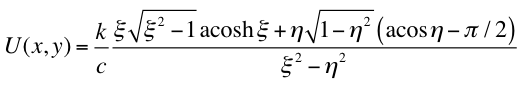
\includegraphics{nllens_potential.png}
%nllens_potential
\[
U(x,y)=\frac{k}{c}\frac{\xi\sqrt{\xi^2-1} \, \text{acosh}\xi + \eta\sqrt{1-\eta^2}(\text{acos}\eta-\pi/2)}{\xi^2-\eta^2}
\]
\\ where 
%%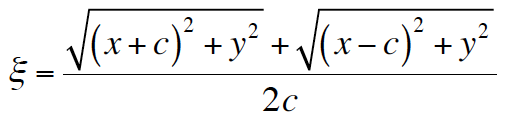
\includegraphics{nllens_xi.png}, 
%%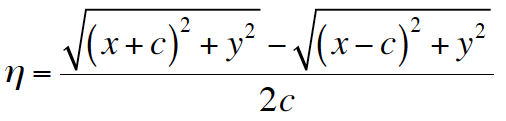
\includegraphics{nllens_eta.png}, and \textit{k} = KNLL, \textit{c} = CNLL. 
%nllens_xi
\[
\xi = \frac{\sqrt{(x+c)^2+y^2}+\sqrt{(x-c)^2+y^2}}{2c}, \quad \eta = \frac{\sqrt{(x+c)^2+y^2}-\sqrt{(x-c)^2+y^2}}{2c},
\]
and \textit{k} = KNLL, \textit{c} = CNLL.

Figure below shows the contour plot of the scalar potential:
\\
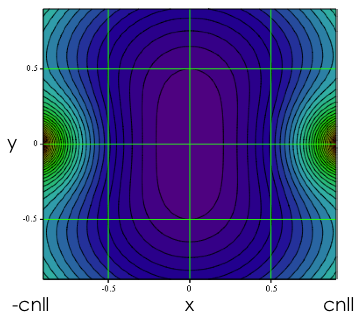
\includegraphics[width=220px]{Introduction/nllens_potential-2D.png}

The multipole expansion of the scalar potential is
\\
%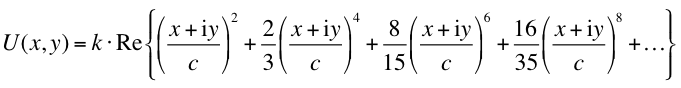
\includegraphics{Introduction/nllens_potential-expansion.png}
%nllens_potential-expansion
\[
U(x,y)=k\cdot Re\left\{ \left(\dfrac{x + i y}{c}\right)^2 + \frac{2}{3}\left(\dfrac{x + i y}{c}\right)^4 + \frac{8}{15}\left(\dfrac{x + i y}{c}\right)^6 + \frac{16}{35}\left(\dfrac{x + i y}{c}\right)^8 + \cdots \right\}
\]
\\ Note that this expansion is only valid inside the \textit{r=c} circle on the x,y plane.   

In order to create integrable optics, one needs to shape the potential along z axis according to the beta-function. Below is an example nonlinear section representing the necessary nonlinear field with 20 thin lenses: 
\begin{verbatim}

    mu0=0.3;  ! phase advance over straight section
    l0=2.0;   ! length of the straight section
    nn=20;    !number of nonlinear elements
    tn=0.45;  ! strength of nonlinear lens
    cn=0.01;  ! dimentional parameter of nonlinear lens

    musect=mu0+0.5;
    f0=l0/4.0*(1.0+1.0/tan(pi*mu0)^2);
    betae=l0/sqrt(1.0-(1.0-l0/2.0/f0)^2);
    alfae=l0/2.0/f0/sqrt(1.0-(1.0-l0/2.0/f0)^2);
    betas=l0*(1-l0/4.0/f0)/sqrt(1.0-(1.0-l0/2.0/f0)^2);
    value,f0,betae,alfae,betas;

ncreate(ii,kk,cc): macro = {n.ii: nllens, knll=kk, cnll=cc;};
i=0;
while(i <  nn)
    {
    i=i+1;
    sn=l0/nn*(i-0.5);
    bn=l0*(1-sn*(l0-sn)/l0/f0)/sqrt(1.0-(1.0-l0/2.0/f0)^2);
    knn=l0*tn*cn^2/nn/bn;
    cnn=cn*sqrt(bn);
    exec,ncreate($i,knn,cnn);
    value,i,bn,cnn,knn;
    };

\end{verbatim}
References:

\begin{enumerate}
	\item V. Danilov, S. Nagaitsev, Phys. Rev. ST Accel. Beams \textbf{13}, 084002 (2010).
    
	\item A. Valishev, S. Nagaitsev, V. Kashikhin, V. Danilov, in Proceedings of 2011 Particle Accelerator Conference, New York, NY, USA, WEP070.

\end{enumerate}
A. Valishev, March 19, 2012


%%\end{document}

\subsection{Nonlinear Lens with Elliptic Potential}
\madbox{
label: NLLENS, KNLL = real, CNLL = real;
}

The NLLENS element represents a thin nonlinear lens with the potential
of 'Elliptic' type as specified in [1]. The lens is used to create fully
integrable 2D nonlinear accelerator lattice with very large nonlinear
tune spread/shift. The NLLENS element is recognized by the thin tracking
module. The quadrupole term of the potential is included in the
TRANSPORT map and, consequently, effects the calculation of tunes and
Twiss functions.   

\begin{madlist}
   \ttitem{KNLL} The integrated strength of lens (m). The strength is
     parametrized so that the quadrupole term of the multipole
     expansion is k1=2*KNLL/CNLL\textasciicircum2.      
   \ttitem{CNLL} The dimensional parameter of lens (m). The singularities
     of the potential are located at X=-CNLL,+CNLL and Y=0.  
\end{madlist}

The scalar potential function of the element is given by
\\
%%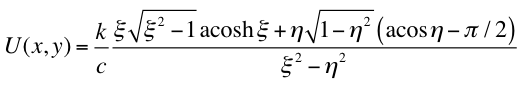
\includegraphics{nllens_potential.png}
%nllens_potential
\[
U(x,y)=\frac{k}{c}\frac{\xi\sqrt{\xi^2-1} \, \text{acosh}\xi +  
  \eta\sqrt{1-\eta^2}(\text{acos}\eta-\pi/2)}{\xi^2-\eta^2}
\]
\\ where \textit{k} = KNLL, \textit{c} = CNLL and 
%%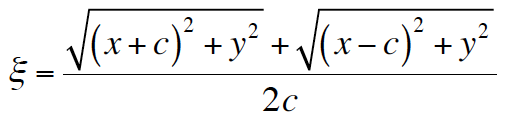
\includegraphics{nllens_xi.png}, 
%%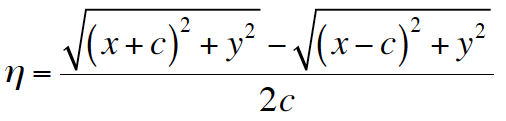
\includegraphics{nllens_eta.png}, and \textit{k} = KNLL, \textit{c} = CNLL. 
%nllens_xi
\[
\xi = \frac{\sqrt{(x+c)^2+y^2}+\sqrt{(x-c)^2+y^2}}{2c}, 
\quad \eta = \frac{\sqrt{(x+c)^2+y^2}-\sqrt{(x-c)^2+y^2}}{2c},
\]


Figure below shows the contour plot of the scalar potential: \\
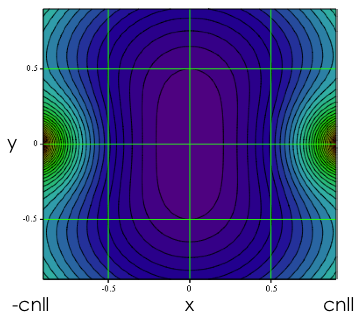
\includegraphics[width=220px]{Introduction/nllens_potential-2D.png}

The multipole expansion of the scalar potential is \\
%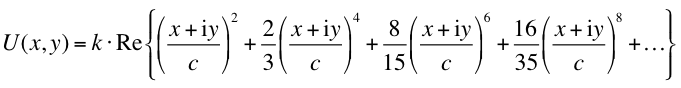
\includegraphics{Introduction/nllens_potential-expansion.png}
%nllens_potential-expansion
\[
U(x,y)=k\cdot Re\left\{ \left(\dfrac{x + i y}{c}\right)^2 + 
\frac{2}{3}\left(\dfrac{x + i y}{c}\right)^4 +
\frac{8}{15}\left(\dfrac{x + i y}{c}\right)^6 + 
\frac{16}{35}\left(\dfrac{x + i y}{c}\right)^8 + \cdots \right\}
\]
\\ 
Note that this expansion is only valid inside the \textit{r=c} circle on
the x,y plane.    

In order to create integrable optics, one needs to shape the potential
along z axis according to the beta-function. Below is an example
nonlinear section representing the necessary nonlinear field with 20
thin lenses:  
\begin{verbatim}
    mu0 = 0.3;  ! phase advance over straight section
    l0 = 2.0;   ! length of the straight section
    nn = 20;    ! number of nonlinear elements
    tn = 0.45;  ! strength of nonlinear lens
    cn = 0.01;  ! dimentional parameter of nonlinear lens

    musect = mu0 + 0.5;
    f0 = l0/4.0*(1.0+1.0/tan(pi*mu0)^2);
    betae = l0/sqrt(1.0-(1.0-l0/2.0/f0)^2);
    alfae = l0/2.0/f0/sqrt(1.0-(1.0-l0/2.0/f0)^2);
    betas = l0*(1-l0/4.0/f0)/sqrt(1.0-(1.0-l0/2.0/f0)^2);
    value, f0, betae, alfae, betas;

    ncreate(ii,kk,cc): macro = {n.ii: nllens, knll=kk, cnll=cc;};

    i=0;
    while(i <  nn)
      {
        i = i+1;
        sn = l0/nn*(i-0.5);
        bn = l0*(1-sn*(l0-sn)/l0/f0)/sqrt(1.0-(1.0-l0/2.0/f0)^2);
        knn = l0*tn*cn^2/nn/bn;
        cnn = cn*sqrt(bn);
        exec, ncreate($i,knn,cnn);
        value, i, bn, cnn, knn;
      };
\end{verbatim}


%% To be moved in References at the end of the document
References:
\begin{enumerate}
\item V. Danilov, S. Nagaitsev, Phys. Rev. ST Accel. Beams \textbf{13},
  084002 (2010). 
  
\item A. Valishev, S. Nagaitsev, V. Kashikhin, V. Danilov, in
  Proceedings of 2011 Particle Accelerator Conference, New York, NY,
  USA, WEP070. 
\end{enumerate}

%A. Valishev, March 19, 2012


%%%\title{KICK, HKICK, VKICK}
%  Changed by: Chris ISELIN, 27-Jan-1997 
%  Changed by: Hans Grote, 30-Sep-2002 
%  Changed by: Frank Schmidt, 28-Aug-2003 
%  Changed by: Werner Herr, 22-May-2007 

\section{Closed Orbit Correctors}
  
Three types of closed orbit correctors are available: 
\begin{itemize}
   \item \href{hkick}{HKICKER}, a corrector for the horizontal plane, 
   \item \href{vkick}{VKICKER}, a corrector for the vertical plane, 
   \item \href{kick}{KICKER}, a corrector for both planes. 
\end{itemize}

\begin{verbatim}
label: HKICKER, L = real, KICK = real, TILT = real;
label: VKICKER, L = real, KICK = real, TILT = real;
label:  KICKER, L = real, HKICK = real, VKICK = real, TILT = real;
\end{verbatim} 

{\bf The type KICKER should not be used when an orbit corrector kicks
  only in one plane.}  

The attributes have the following meaning: 
\begin{itemize}
   \item L: The length of the closed orbit corrector (default: 0 m). 
   \item KICK: The kick angle for either horizontal or vertical correctors. (default: 0 rad). 
   \item HKICK: The horizontal kick angle for a corrector in both planes (default: 0 rad). 
   \item VKICK: The vertical kick angle for a corrector in both planes (default: 0 rad). 
   \item TILT: The roll angle about the longitudinal axis (default: 0
     rad). A positive angle represents a clockwise rotation of the
     kicker.  
\end{itemize} 

A positive kick increases \textit{p$_x$} or \textit{p$_y$}
respectively. This means that a positive horizontal kick bends to the
left,  i.e. to positive x which is opposite of what is true for bends.   

It should be noted that the kick values assigned to an orbit corrector
like above are not overwritten by an orbit correction using the CORRECT
command. Instead the kicks computed by an orbit correction and the
assigned values are added when the correctors are used.  

 Examples: 
\begin{verbatim}
HK1:   HKICKER, KICK = 0.001;
VK3:   VKICKER, KICK = 0.0005;
VK4:   VKICKER, KICK := AVK4;
KHV1:  KICKER,  HKICK = 0.001, VKICK = 0.0005;
KHV2:  KICKER,  HKICK := AKHV2H, VKICK := AKHV2V;
\end{verbatim} 

The assignment in the form of a deferred expression has the advantage
that the values can be assigned and/or modified at any time (and matched
!).  

The \href{local_system.html#straight}{straight reference system} for an
orbit corrector is a Cartesian coordinate s ystem.  

Please note that there is a new feature introduced by Stefan Sorge from
GSI. Here his decription:

The elements KICKER, HKICKER, and VKICKER can also be used as  an
exciter providing a sinusoidal momentum kick. The usage in this case is   

\begin{verbatim}
xykick: KICKER,  SINKICK = integer, SINPEAK = real, SINTUNE = real, SINPHASE = real;  
xkick : HKICKER, SINKICK = integer, SINPEAK = real, SINTUNE = real, SINPHASE = real;  
ykick : VKICKER, SINKICK = integer, SINPEAK = real, SINTUNE = real, SINPHASE = real;  
\end{verbatim}
where a sinusoidal momentum kick dpz as a function of the  revolution
number n given by\\   
dpz(n)=SINPEAK * sin(2*PI*SINTUNE*n + SINPHASE), pz=px,py \\ 
is provided. 

The variables are 

\begin{itemize}
   \item SINKICK - integer, must be set to 1 to switch on the sinusoidal
     signal, default: 0.  
   \item SINPEAK - amplitude of the bending angle (rad), default: 0 rad.  
   \item SINTUNE - frequency of the signal times the revolution
     frequency.  Hence, the phase per revolution is 2*PI*SINTUNE,
     default: 0.   
   \item SINPHASE - initial phase, default: 0 rad.  
   \item KICKER generates a kick in horizontal and a kick vertical
     direction,  where both are synchron, HKICKER generates a horizontal
     kick,  and VKICKER generates a vertical kick.   
\end{itemize}

The momentum kick of a kicker has only a single frequency. An element
having a finite bandwidth can approximately created by defining  thin
kickers with all amplitudes SINPEAK, frequencies SINTUNE, and  initial
phases SINPHASE desired and putting them at the same position s in  the
accelerator.   

From S.Sorge@gsi.de  

%\href{http://www.cern.ch/Hans.Grote/hansg_sign.html}{hansg}, 
%\href{http://www.cern.ch/Frank.Schmidt/frs_sign.html}{frs}, August 28, 2003  

%  Changed by: Frank Schmidt, 28-Aug-2003 
%  Changed by: Werner Herr, 22-May-2007 
\subsection{Closed Orbit Correctors}
\label{sec:closed_orbit_cor}
Three types of closed orbit correctors are available: 
\begin{madlist}
   \ttitem{\href{hkick}{HKICKER}} a corrector for the horizontal plane, 
   \ttitem{\href{vkick}{VKICKER}} a corrector for the vertical plane, 
   \ttitem{\href{kick}{KICKER}} a corrector for both planes. 
\end{madlist}

\madbox{
xxxxxxxxxxxxxxxxx\=xxxxxxxxxxxxxxxxxxxxxxxx\= \kill
label: HKICKER, \>L = real, KICK = real, \>TILT = real; \\
label: VKICKER, \>L = real, KICK = real, \>TILT = real; \\
label: KICKER,  \>L = real, HKICK = real, \>VKICK = real, TILT = real;
}

{\bf The type KICKER should not be used when an orbit corrector kicks
  only in one plane.}  

The attributes have the following meaning: 
\begin{madlist}
   \ttitem{L} The length of the closed orbit corrector (default: 0 m). 
   \ttitem{KICK} The momentum change $\delta PX = \delta p_x/p_0$ or 
     $\delta PY = \delta p_y / p_0$ for respectively horizontal or vertical
     correctors. (default: 0).  
   \ttitem{HKICK} The horizontal momentum change 
     $\delta PX = \delta p_x/p_0$ for a corrector acting in both planes
     (default: 0).  
   \ttitem{VKICK} The vertical momentum change 
     $\delta PY = \delta p_y/p_0$  for a corrector acting in both planes
     (default: 0).  
   \ttitem{TILT} The roll angle about the longitudinal axis (default: 0
     rad). A positive angle represents a clockwise rotation of the
     kicker.  
\end{madlist}

A positive kick increases $p_x$ or $p_y$ respectively. This
means that a positive horizontal kick bends to the left,  i.e. to
positive $x$ which is opposite of what is true for bends.    

The deviation angle $\theta$ of the particle trajectory is related to
the momentum change through  $\sin \theta = \delta P = \delta p / p_0$.

It should be noted that the kick values assigned to an orbit corrector
like above are not overwritten by an orbit correction using the CORRECT
command. Instead the kicks computed by an orbit correction and the
assigned values are added when the correctors are used.  

 Examples: 
\madxmp{
xxxxxxx\=xxxxxxxxxx\=xxxxxxxxxxxxxxxxx\= \kill
HK1:   \>HKICKER, \>KICK = 0.001;  \\
VK3:   \>VKICKER, \>KICK = 0.0005; \\
VK4:   \>VKICKER, \>KICK := AVK4; \\
KHV1:  \>KICKER,  \>HKICK = 0.001,   \>VKICK = 0.0005; \\
KHV2:  \>KICKER,  \>HKICK := AKHV2H, \>VKICK := AKHV2V;
}

The assignment in the form of a deferred expression has the advantage
that the values can be assigned and/or modified at any time (and
matched!).   

The \href{local_system.html#straight}{straight reference system} for an
orbit corrector is a Cartesian coordinate s ystem.  



Please note that there is a new feature introduced by Stefan Sorge from
GSI. Here his decription:

The elements KICKER, HKICKER, and VKICKER can also be used as  an
exciter providing a sinusoidal momentum kick. The usage in this case is   

\madxmp{
xykick: KICKER,  \= SINKICK=integer, SINPEAK=real, SINTUNE=real, SINPHASE=real;  \\
xkick : HKICKER, \> SINKICK=integer, SINPEAK=real, SINTUNE=real, SINPHASE=real;  \\
ykick : VKICKER, \> SINKICK=integer, SINPEAK=real, SINTUNE=real, SINPHASE=real;  
}
where a sinusoidal momentum kick dpz as a function of the  revolution
number n given by\\   
dpz(n)=SINPEAK * sin(2*PI*SINTUNE*n + SINPHASE), pz=px,py \\ 
is provided. 

The KICKER element generates synchronous kicks in both horizontal and
vertical planes. HKICKER generates only a horizontal kick, and VKICKER
generates only a vertical kick.   

The variables are 

\begin{madlist}
   \ttitem{SINKICK} must be set to 1 to switch on the sinusoidal
     signal, default: 0.  
   \ttitem{SINPEAK} amplitude of the bending angle (rad); default: 0
     rad.   
   \ttitem{SINTUNE} frequency of the signal times the revolution
     frequency.  Hence, the phase per revolution is 2*PI*SINTUNE;
     default: 0.   
   \ttitem{SINPHASE} initial phase; default: 0 rad.  
\end{madlist}

The momentum kick of a kicker has only a single frequency. An element
having a finite bandwidth can approximately created by defining  thin
kickers with all amplitudes SINPEAK, frequencies SINTUNE, and  initial
phases SINPHASE desired and putting them at the same position s in  the
accelerator.   

%From S.Sorge@gsi.de  


%%%\title{TKICK}
%  Created by: Laurent Deniau, 15-Sep-2011 

%%\usepackage{hyperref}
% commands generated by html2latex


%%\begin{document}
%%\begin{center}
 %%EUROPEAN ORGANIZATION FOR NUCLEAR RESEARCH 
%%\includegraphics{http://cern.ch/madx/icons/mx7_25.gif}

\subsection{Transverse Kicker}
%%\end{center}

 The type TKICKER should be used to create horizontal, vertical or combined transverse kickers physically equivalent to elements of type KICKER, but \textbf{not used} by the closed orbit correction module (see \href{../cororbit/co_correct.html}{CORRECT} command).  

Examples of elements that may use the type TKICKER: 
\begin{itemize}
	\item Fast kickers for injection, dump \& tune
	\item Magnetic septa towards beam dump
	\item Dampers of transverse beam oscillations
	\item Undulator \& Wiggler magnets
\end{itemize}

 For further information on element type TKICKER and its attributes, look at the documentation of the orbit corrector type \href{kickers.html#kick}{KICKER}.  

\href{mailto:mad@cern.ch}{madx team}, September 15, 2011  

%%\end{document}

%  Created by: Laurent Deniau, 15-Sep-2011 
\subsection{Transverse Kicker}
The type TKICKER should be used to create horizontal, vertical or
combined transverse kickers physically equivalent to elements of type
KICKER, but \textbf{not used} by the closed orbit correction module (see
\href{../cororbit/co_correct.html}{CORRECT} command).   

Examples of elements that may use the type TKICKER: 
\begin{itemize}
   \item Fast kickers for injection, dump \& tune
   \item Magnetic septa towards beam dump
   \item Dampers of transverse beam oscillations
   \item Undulator \& Wiggler magnets
\end{itemize}

For further information on element type TKICKER and its attributes, look
at the documentation of the orbit corrector type
\href{kickers.html#kick}{KICKER}.   

%\href{mailto:mad@cern.ch}{madx team}, September 15, 2011  


%%%\title{RFCAVITY}
%  Changed by: Chris ISELIN, 27-Jan-1997 
%  Changed by: Hans Grote, 30-Sep-2002 

\section{RF Cavity}


\begin{verbatim}
label: RFCAVITY, L = real, VOLT = real, LAG = real, HARMON = integer, FREQ = real;                  
\end{verbatim} 

%  HARMON=integer, BETRF=real,PG=real,
%                  FREQ=real,SHUNT=real,TFILL=real; 


An RFCAVITY has eight real attributes and one integer attribute: 
\begin{itemize}
   \item L: The length of the cavity (DEFAULT: 0 m) 
   \item VOLT: The peak RF voltage (DEFAULT: 0 MV). The effect of the cavity is \\
     delta(\textit{E}) = VOLT * sin(2 pi * (LAG - HARMON * \textit{f$_0$ t})). 
   \item LAG: The phase lag [2pi] (DEFAULT: 0). 
   \item FREQ: The frequency [MHz] (no DEFAULT). Note that if the RF
     frequency is not given, it is computed from the harmonic number and
     the revolution frequency \textit{f$_0$} as before. However, for
     accelerating structures this makes no sense, and the frequency is
     mandatory.  
   \item HARMON: The harmonic number \textit{h} (no DEFAULT). Only if
     the frequency is not given.  
   \item \textit{ Please take note, that the following MAD8 attributes:
     BETRF, PG, SHUNT and TFILL are currently not implemented in MAD-X!}    
%  \item BETRF: RF coupling factor (DEFAULT: 0).
%  \item PG: The RF power per cavity (DEFAULT: 0 MW).
%  \item SHUNT: The relative shunt impedance (DEFAULT: 0 MOhm/m).
%  \item TFILL: The filling time of the cavity $T_{fill}$ (DEFAULT: 0 microseconds). 

   \item \textit{ Note as well that twiss is 4D only. As a consequence
     the TWISS parameters in the plane of non-zero dispersion may not
     close as expected. Therefore, it is best to perform TWISS in 4D
     only, i.e. with cavities switched off. If 6D is needed one has to
     use the \href{../ptc_twiss/ptc_twiss.html}{ptc\_twiss} command. } 
\end{itemize}  

The RFCAVITY has attributes that will only become active in PTC: 
\begin{itemize}
   \item n\_bessel (DEFAULT: 0): \\
     Transverse focussing effects are typically ignored in the cavity in
     MAD-X or even PTC. This effect is being calculated to order n\_bessel,
     with n\_bessel=0 disregarding this effect and with a correct treatment
     when n\_bessel goes to infinty.
   \item no\_cavity\_totalpath (DEFAULT: no\_cavity\_totalpath=false): \\
     flag to choose if in a cavity the transit time factor is considered
     (no\_cavity\_totalpath=false) or if the particle is kept on the
     crest of RF voltage (no\_cavity\_totalpath=true).  
\end{itemize}  

A cavity requires the particle energy (\href{beam.html#energy}{ENERGY})
and the particle charge (\href{beam.html#charge}{CHARGE}) to be set by a
\href{beam.html}{BEAM} command before any calculations are performed.  

 Example: 
\begin{verbatim}
BEAM, PARTICLE = ELECTRON, ENERGY = 50.0;
CAVITY: RFCAVITY, L = 10.0, VOLT = 150.0, LAG = 0.0, HARMON = 31320;
\end{verbatim} 

The \href{local_system.html#straight}{straight reference system} for a
cavity is a cartesian coordinate system.  

%\href{http://www.cern.ch/Hans.Grote/hansg_sign.html}{hansg}, January 24, 1997 

\subsection{RF Cavity}
\label{sec:rf_cavity}

\madbox{
label: RFCAVITY, \= L = real, VOLT = real, LAG = real, \\
                 \> HARMON = integer, FREQ = real, \\    
                 \> N\_BESSEL = integer, NO\_CAVITY\_TOTALPATH = logical;
}

%  HARMON=integer, BETRF=real,PG=real,
%                  FREQ=real,SHUNT=real,TFILL=real; 


An RFCAVITY has eight real attributes and one integer attribute: 
\begin{madlist}
   \ttitem{L} The length of the cavity (DEFAULT: 0 m) 
   \ttitem{VOLT} The peak RF voltage (DEFAULT: 0 MV). The effect of the cavity is \\
     delta(\textit{E}) = VOLT * sin(2 pi * (LAG - HARMON * \textit{f$_0$ t})). 
   \ttitem{LAG} The phase lag [2pi] (DEFAULT: 0). 
   \ttitem{FREQ} The frequency [MHz] (no DEFAULT). Note that if the RF
     frequency is not given, it is computed from the harmonic number and
     the revolution frequency \textit{f$_0$} as before. However, for
     accelerating structures this makes no sense, and the frequency is
     mandatory.  
   \ttitem{HARMON} The harmonic number \textit{h} (no DEFAULT). Only if
     the frequency is not given.  
\end{madlist}

\textit{ Please take note, that the following \madeight attributes:
  BETRF, PG, SHUNT and TFILL are currently not implemented in \madx!}    
%  \item BETRF: RF coupling factor (DEFAULT: 0).
%  \item PG: The RF power per cavity (DEFAULT: 0 MW).
%  \item SHUNT: The relative shunt impedance (DEFAULT: 0 MOhm/m).
%  \item TFILL: The filling time of the cavity $T_{fill}$ (DEFAULT: 0 microseconds). 

\textit{ Note as well that twiss is 4D only. As a consequence
  the TWISS parameters in the plane of non-zero dispersion may not
  close as expected. Therefore, it is best to perform TWISS in 4D
  only, i.e. with cavities switched off. If 6D is needed one has to
  use the \href{../ptc_twiss/ptc_twiss.html}{ptc\_twiss} command. } 

The RFCAVITY can also have attributes that will only become active in PTC: 
\begin{madlist}
   \ttitem{N\_BESSEL} (DEFAULT: 0): \\
     Transverse focussing effects are typically ignored in the cavity in
     \madx or even PTC. This effect is being calculated to order n\_bessel,
     with n\_bessel=0 disregarding this effect and with a correct treatment
     when n\_bessel goes to infinty.
   \ttitem{NO\_CAVITY\_TOTALPATH} (DEFAULT: no\_cavity\_totalpath=false): \\
     flag to select whether the transit time factor in the cavity is to be
     considered (no\_cavity\_totalpath = false) or if the particle is
     kept on the crest of RF voltage (no\_cavity\_totalpath = true).  
\end{madlist}

A cavity requires the particle energy (\href{beam.html#energy}{ENERGY})
and the particle charge (\href{beam.html#charge}{CHARGE}) to be set by a
\href{beam.html}{BEAM} command before any calculations are performed.  

 Example: 
\madxmp{
BEAM, PARTICLE = ELECTRON, ENERGY = 50.0; \\
CAVITY: RFCAVITY, L = 10.0, VOLT = 150.0, LAG = 0.0, HARMON = 31320;
}

The \href{local_system.html#straight}{straight reference system} for a
cavity is a cartesian coordinate system.  


%%%\title{MULTIPOLE}
%  Changed by: Chris ISELIN, 27-Jan-1997 
%  Changed by: Hans Grote, 17-Jun-2002 
%  Changed by: Frank Schmidt, 28-Aug-2003 

\section{RFMULTIPOLE: Thin Radio-Frequency Multipole}
\begin{verbatim}
Label: RFMULTIPOLE, VOLT = real, LAG = real,
       HARMON = integer, FREQ = real,
       LRAD = real, TILT = real,
       KNL := {k0nl, k1nl, k2nl, ... },  ! Normal coefficients
       KSL := {k0sl, k1sl, k2sl, ... },  ! Skew coefficients
       PNL := {p0n,  p1n,  p2n,  ... },  ! Normal phases [2pi]
       PSL := {p0s,  p1s,  p2s,  ... };  ! Skew phases [2pi]
\end{verbatim} 

A RFMULTIPOLE is a thin-lens element which exhibits the properties
of an RF-cavity and of a magnet of arbitrary order oscillating the
a certain frequency:        
 
\begin{itemize}
   \item L: The length of the rfmultipole (DEFAULT: 0 m) 
   \item LAG: The phase lag [2pi] (DEFAULT: 0) 
   \item FREQ: The frequency [MHz] (no DEFAULT). Note that if the RF
     frequency is not given, it is computed from the harmonic
     number and the revolution frequency f0 as before. However, for
     accelerating structures this makes no sense, and the frequency
     is mandatory.  
   \item HARMON: The harmonic number h (no DEFAULT). Only if the
     frequency is not given. 
   \item LRAD: A fictitious length, which was originally just used to
     compute synchrotron radiation effects. A non-zero LRAD in
     conjunction with the OPTION thin\_foc set to a true logical value
     takes into account of the weak focussing of bending magnets.  
   \item TILT: The roll angle about the longitudinal axis (default: 0
     rad). A positive angle represents a clockwise rotation of the
     multipole element.            

     \textbf{Please note that contrary to MAD8 one has to specify the
       desired TILT angle, otherwise it is taken as 0 rad. We
       believe that the MAD8 concept of having individual TILT
       values for each component and on top with default values
       led to considerable confusion and allowed for excessive
       and unphysical freedom. Instead, in MAD-X the KNL/KSL
       components can be considered as the normal or skew
       multipole components of the magnet on the bench, while the
       TILT attribute can be considered as an tilt alignment
       error in the machine.} 

   \item KNL: The normal rfmultipole coefficients from order zero to
     the maximum; the parameters are positional, therefore zeros
     must be filled in for components that do not exist. Example of
     a thin-lens sextupole: ms:rfmultipole, knl:=\{0, 0, k2l\}; 
   \item KSL: The skew rfmultipole coefficients from order zero to
     the maximum; the parameters are positional, therefore zeros
     must be filled in for components that do not exist. Example of
     a thin-lens skew octupole:
\end{itemize}

\begin{verbatim}
ms: rfmultipole, ksl := {0, 0, 0, k3sl};
\end{verbatim}

Both KNL and KSL may be specified for the same multipole.  


\begin{itemize}
   \item VOLT: The peak RF voltage (DEFAULT: 0 MV). The effect of the
     cavity is \\ 
     delta(E) = VOLT * sin(2 pi * (LAG - HARMON * f0 t)). 
   \item PNL: The phase for each normal rfmultipole coefficients from
     order zero to the maximum; the parameters are positional,
     therefore zeros must be filled in for components that do not
     exist.  
   \item PSL: The phase for each skew rfmultipole coefficients from
     order zero to the maximum; the parameters are positional,
     therefore zeros must be filled in for components that do not
     exist.  
\end{itemize}       

A rfmultipole requires the particle energy (ENERGY) and the
particle charge (CHARGE) to be set by a BEAM command before any
calculations are performed. Notice that, contrary to the regular
multipole where the dipole component has no effect on the
reference orbit, an RF-Multipole that includes a dipole component
bends also the reference orbit.      


%\href{https://phonebook.cern.ch/foundpub/Phonebook/index.html?search=latina#id=PE525753}{Andrea
%Latina}, September 28, 2012  

\subsection{Thin Radio-Frequency Multipole}
\madbox{
xxxxxxxxxxxxxxxxxxxxx\=xxxxxxxxxxxxxxxxxxxxxxxxxxxxxxx\= \kill
label: RFMULTIPOLE, \> VOLT = real, LAG = real, \\
       \> HARMON = integer, FREQ = real, \\
       \> LRAD = real, TILT = real, \\
       \> KNL := \{k0nl, k1nl, k2nl, \ldots \}, \>!Normal coefficients \\
       \> KSL := \{k0sl, k1sl, k2sl, \ldots \}, \>!Skew coefficients \\
       \> PNL := \{p0n,  p1n,  p2n,  \ldots \}, \>!Normal phases [2pi] \\
       \> PSL := \{p0s,  p1s,  p2s,  \ldots \}; \>!Skew phases [2pi]
}

A RFMULTIPOLE is a thin-lens element which exhibits the properties
of an RF-cavity and of a magnet of arbitrary order oscillating the
a certain frequency:        

The effect of the cavity is delta(E) = VOLT * sin(2 pi * (LAG - HARMON *
f0 t)). 
 
\begin{madlist}
%   \ttitem{L} The length of the rfmultipole (DEFAULT: 0 m) 
   \ttitem{VOLT} The peak RF voltage (DEFAULT: 0 MV).  
   \ttitem{LAG} The phase lag [2pi] (DEFAULT: 0) 
   \ttitem{FREQ} The frequency [MHz] (no DEFAULT). \\ 
     Note that if the RF
     frequency is not given, it is computed from the harmonic
     number and the revolution frequency f0 as before. However, for
     accelerating structures this makes no sense, and the frequency
     is mandatory.  
   \ttitem{HARMON} The harmonic number h (no DEFAULT). Only if the
     frequency is not given. 
   \ttitem{LRAD} A fictitious length, which was originally just used to
     compute synchrotron radiation effects. A non-zero LRAD in
     conjunction with the OPTION thin\_foc set to a true logical value
     takes into account of the weak focussing of bending magnets.  
   \ttitem{TILT} The roll angle about the longitudinal axis (default: 0
     rad). A positive angle represents a clockwise rotation of the
     multipole element.            

     \textbf{Please note that contrary to \madeight one has to specify the
       desired TILT angle, otherwise it is taken as 0 rad. We
       believe that the \madeight concept of having individual TILT
       values for each component and on top with default values
       led to considerable confusion and allowed for excessive
       and unphysical freedom. Instead, in \madx the KNL/KSL
       components can be considered as the normal or skew
       multipole components of the magnet on the bench, while the
       TILT attribute can be considered as an tilt alignment
       error in the machine.} 

   \ttitem{KNL} The normal rfmultipole coefficients from order zero to
     the maximum; the parameters are positional, therefore zeros
     must be filled in for components that do not exist. Example of
     a thin-lens sextupole: ms:rfmultipole, knl:=\{0, 0, k2l\}; 
   \ttitem{KSL} The skew rfmultipole coefficients from order zero to
     the maximum; the parameters are positional, therefore zeros
     must be filled in for components that do not exist. Example of
     a thin-lens skew octupole:

   \ttitem{PNL} The phase for each normal rfmultipole coefficients from
     order zero to the maximum; the parameters are positional,
     therefore zeros must be filled in for components that do not
     exist.  
   \ttitem{PSL} The phase for each skew rfmultipole coefficients from
     order zero to the maximum; the parameters are positional,
     therefore zeros must be filled in for components that do not
     exist.  
\end{madlist}


Example:
\madxmp{ms: rfmultipole, ksl := \{0, 0, 0, k3sl\};}

Both KNL and KSL may be specified for the same multipole.  

A rfmultipole requires the particle energy (ENERGY) and the
particle charge (CHARGE) to be set by a BEAM command before any
calculations are performed. Notice that, contrary to the regular
multipole where the dipole component has no effect on the
reference orbit, an RF-Multipole that includes a dipole component
bends also the reference orbit.      


%\href{https://phonebook.cern.ch/foundpub/Phonebook/index.html?search=latina#id=PE525753}{Andrea
%Latina}, September 28, 2012  

%%%\title{CRABCAVITY}
%  Added by: R. Calaga, Sep 2010 
%  Edited by: A. Latina, Jun 2013

\section{Crab Cavity}


\begin{verbatim}
label: CRABCAVITY, L = real, VOLT = real, LAG = real, FREQ = real,
                   RV1 = integer, RV2 = integer, RV3 = integer, RV4 = integer, 
                   RPH1 = integer, RPH2 = integer, 
                   LAGF = real, HARMON = integer;                 
\end{verbatim} 

%  BETRF=real, PG=real,
%  FREQ=real, SHUNT=real, TFILL=real; 

A CRABCAVITY has five real attributes and seven integer attributes: 

\begin{itemize}
  \item L: The length of the cavity (default: 0 m) 

  \item VOLT: The peak RF voltage (default: 0 MV). 

  \item LAG: The initial phase lag [2pi] (default: 0). 

  \item FREQ: The RF frequency [MHz] (no default). \\
    {\bf Note that if the RF frequency is not given, it is computed from the
    harmonic number and the revolution frequency \textit{f$_0$} as before. 
    However, for deflecting structures this makes no sense, and the 
    frequency is mandatory.} 

  \item RV1: Number of initial turns with zero voltage (default: 0). 
  \item RV2: Number of turns to ramp voltage from zero to nominal value (default: 0). 
  \item RV3: Number of turns with nominal voltage (default: 0). 
  \item RV4: Number of turns to ramp voltage from nominal value to zero (default: 0).  

  \item LAGF: Value of the final crab RF phase lag [2pi] (default: 0).

  \item RPH1: Number of initial turns with nominal phase (default: 0). 
  \item RPH2: Number of turns to ramp phase [2pi] from nominal to
    specified value \\ (default:~0). 

  \item HARMON: The harmonic number \textit{h} (no default). \\
    Only if the frequency is not given. 

% \item BETRF: RF coupling factor (default: 0).
% \item PG: The RF power per cavity (default: 0 MW).
% \item SHUNT: The relative shunt impedance (default: 0 MOhm/m).
% \item TFILL: The filling time of the cavity T<sub>fill</sub> (default: 0 microseconds). 
%\item EPHASE: Value of the final crab RF phase [2pi] with respect to  nominal value (default: 0). 
\end{itemize}


{\bf Caveats:}
\begin{itemize}
   \item \textit{ Please take note, that the following MAD8 attributes:
     BETRF, PG, SHUNT and TFILL are currently not implemented in MAD-X!}
   \item \textit{ Note that crab cavities are only implemented for
     tracking  purposes. \\ TWISS will ignore any effect of the crab cavity.  
% as well that twiss is 4D only. As a consequence the TWISS
% parameters in the plane of non-zero dispersion may not close as
% expected. Therefore, it is best to perform TWISS in 4D only, i.e. with
% cavities switched off. If 6D is needed one has to use the
% 
% <a href="../ptc_twiss/ptc_twiss.html">ptc_twiss</a> command. 
}
\end{itemize} 

%A cavity requires the particle energy (\href{beam.html#energy}{ENERGY})
%and the particle charge (\href{beam.html#charge}{CHARGE}) to be set by
%a \href{beam.html}{BEAM} command before any calculation is performed. 

Before any calculation is performed with a CRABCAVITY, the particle
energy (\href{beam.html#energy}{ENERGY}) and the particle charge
(\href{beam.html#charge}{CHARGE}) must be set by a
\href{beam.html}{BEAM} command.   

Then the effect of the CRABCAVITY on particle coordinates during tracking is
\\
\\ delta(\textit{px})  = VOLT * sin( PHI - OMEGA * t) 
\\ delta(\textit{E})  = -  VOLT * OMEGA * x * cos(PHI - OMEGA * t) 
\\ 
\\ where PHI =  2 $\pi$ * (LAG - HARMON * \textit{f$_0$ t}), 
\\ and OMEGA = 2 $\pi$ * FREQ / \textit{c}
\\
% delta(<i>E</i>) = VOLT * 
% sin(2 pi * (LAG - HARMON * <i>f<sub>0</sub> t</i>)). 


Example: 
\begin{verbatim}
BEAM, PARTICLE = PROTON, ENERGY = 7000.0;
CAVITY:  CRABCAVITY, L = 10.0, VOLT = 5.0, LAG = 0.0, FREQ = 400,
         RV1 = 0, RV2 = 50, RV3 = 1000, RV4 = 50, 
         RPH1 = 100, RPH2 = 500, LAGF = 0.125;
\end{verbatim} 

The \href{local_system.html#straight}{straight reference system} for a
cavity is a cartesian coordinate system.  
 
%\href{http://www.cern.ch/rcalaga}{R. Calaga}, September 2010

%%\title{CRABCAVITY}
%  Added by: R. Calaga, Sep 2010 
%  Edited by: A. Latina, Jun 2013
\subsection{Crab Cavity}
\label{sec:crab_cavity}

\madbox{
label: CRABCAVITY, \=L=real, VOLT=real, LAG=real, FREQ=real, \\
                   \>RV1=integer, RV2=integer, RV3=integer, RV4=integer, \\
                   \>RPH1=integer, RPH2=integer, \\
                   \>LAGF=real, HARMON=integer;
}

%  BETRF=real, PG=real,
%  FREQ=real, SHUNT=real, TFILL=real; 

A CRABCAVITY has five real attributes and seven integer attributes: 

\begin{madlist}
  \ttitem{L} The length of the cavity (default: 0 m) 

  \ttitem{VOLT} The peak RF voltage (default: 0 MV). 

  \ttitem{LAG} The initial phase lag [2pi] (default: 0). 

  \ttitem{FREQ} The RF frequency [MHz] (no default). \\
    {\bf Note that if the RF frequency is not given, it is computed from the
    harmonic number and the revolution frequency \textit{f$_0$} as before. 
    However, for deflecting structures this makes no sense, and the 
    frequency is mandatory.} 

  \ttitem{RV1} Number of initial turns with zero voltage (default: 0). 
  \ttitem{RV2} Number of turns to ramp voltage from zero to nominal value (default: 0). 
  \ttitem{RV3} Number of turns with nominal voltage (default: 0). 
  \ttitem{RV4} Number of turns to ramp voltage from nominal value to zero (default: 0).  

  \ttitem{LAGF} Value of the final crab RF phase lag [2pi] (default: 0).

  \ttitem{RPH1} Number of initial turns with nominal phase (default: 0). 
  \ttitem{RPH2} Number of turns to ramp phase [2pi] from nominal to
    specified value \\ (default:~0). 

  \ttitem{HARMON} The harmonic number \textit{h} (no default). \\
    Only if the frequency is not given. 

% \item BETRF: RF coupling factor (default: 0).
% \item PG: The RF power per cavity (default: 0 MW).
% \item SHUNT: The relative shunt impedance (default: 0 MOhm/m).
% \item TFILL: The filling time of the cavity T<sub>fill</sub> (default: 0 microseconds). 
%\item EPHASE: Value of the final crab RF phase [2pi] with respect to  nominal value (default: 0). 
\end{madlist}


{\bf Caveats:}
\begin{itemize}
   \item \textit{ Please take note, that the following \madeight attributes:
     BETRF, PG, SHUNT and TFILL are currently not implemented in \madx!}
   \item \textit{ Note that crab cavities are only implemented for
     tracking  purposes. \\ TWISS will ignore any effect of the crab cavity.  
% as well that twiss is 4D only. As a consequence the TWISS
% parameters in the plane of non-zero dispersion may not close as
% expected. Therefore, it is best to perform TWISS in 4D only, i.e. with
% cavities switched off. If 6D is needed one has to use the
% 
% <a href="../ptc_twiss/ptc_twiss.html">ptc_twiss</a> command. 
}
\end{itemize} 

%A cavity requires the particle energy (\href{beam.html#energy}{ENERGY})
%and the particle charge (\href{beam.html#charge}{CHARGE}) to be set by
%a \href{beam.html}{BEAM} command before any calculation is performed. 

Before any calculation is performed with a CRABCAVITY, the particle
energy (\href{beam.html#energy}{ENERGY}) and the particle charge
(\href{beam.html#charge}{CHARGE}) must be set by a
\href{beam.html}{BEAM} command.   

Then the effect of the CRABCAVITY on particle coordinates during tracking is
\\
\\ delta(\textit{px})  = VOLT * sin( PHI - OMEGA * t) 
\\ delta(\textit{E})  = -  VOLT * OMEGA * x * cos(PHI - OMEGA * t) 
\\ 
\\ where PHI =  2 $\pi$ * (LAG - HARMON * \textit{f$_0$ t}), 
\\ and OMEGA = 2 $\pi$ * FREQ / \textit{c}
\\
% delta(<i>E</i>) = VOLT * 
% sin(2 pi * (LAG - HARMON * <i>f<sub>0</sub> t</i>)). 


Example: 
\madxmp{
xxxxxxxx\= \kill
BEAM, PARTICLE = PROTON, ENERGY = 7000.0; \\
CAVITY:  \>CRABCAVITY, L = 10.0, VOLT = 5.0, LAG = 0.0, FREQ = 400, \\
         \>RV1 = 0, RV2 = 50, RV3 = 1000, RV4 = 50, \\
         \>RPH1 = 100, RPH2 = 500, LAGF = 0.125;
}

The \href{local_system.html#straight}{straight reference system} for a
cavity is a cartesian coordinate system.  
 
%\href{http://www.cern.ch/rcalaga}{R. Calaga}, September 2010


%%%\title{ELSEPARATOR}
%  Changed by: Chris ISELIN, 27-Jan-1997 
%  Changed by: Hans Grote, 30-Sep-2002 
%  Changed by: Frank Schmidt, 28-Aug-2003 

\section{ELSEPARATOR: Electrostatic Separator}

\begin{verbatim}
label: ELSEPARATOR, L = real, EX = real, EY = real, TILT = real;
\end{verbatim} 

An ELSEPARATOR (electrostatic separator) has four real attributes: 
\begin{itemize}
   \item L: The length of the separator (default: 0 m). 
   \item EX: The horizontal electric field strength (default: 0 MV/m). 
     A positive field increases \textit{p$_x$} for positive particles.  
   \item EY: The vertical electric field strength (default: 0 MV/m). 
     A positive field increases \textit{p$_y$} for positive particles.  
   \item TILT: The roll angle about the longitudinal axis (default: 0
     rad). A positive angle represents a clockwise of the electrostatic
     separator.  
\end{itemize} 

A separator requires the particle energy
(\href{beam.html#energy}{ENERGY}) and the particle charge
(\href{beam.html#charge}{CHARGE}) to be set by a \href{beam.html}{BEAM}
command before any calculations are performed.  

Example: 
\begin{verbatim}
BEAM,PARTICLE = POSITRON, ENERGY = 50.0;
SEP: ELSEPARATOR, L = 5.0, EY = 0.5;
\end{verbatim} 

The \href{local_system.html#straight}{straight reference system} for a
separator is a cartesian coordinate system.   

%\href{http://www.cern.ch/Hans.Grote/hansg_sign.html}{hansg}, 
%\href{http://www.cern.ch/Frank.Schmidt/frs_sign.html}{frs}, August 28, 2003  

%  Changed by: Frank Schmidt, 28-Aug-2003 
\subsection{Electrostatic Separator}
\label{sec:separator}

\madbox{
label: ELSEPARATOR, L = real, EX = real, EY = real, TILT = real;
}

An ELSEPARATOR has four real attributes: 
\begin{madlist}
   \ttitem{L} The length of the separator (default: 0 m). 
   \ttitem{EX} The horizontal electric field strength (default: 0 MV/m). 
     A positive field increases \textit{p$_x$} for positive particles.  
   \ttitem{EY} The vertical electric field strength (default: 0 MV/m). 
     A positive field increases \textit{p$_y$} for positive particles.  
   \ttitem{TILT} The roll angle about the longitudinal axis (default: 0
     rad). A positive angle represents a clockwise of the electrostatic
     separator.  
\end{madlist}

A separator requires the particle energy
(\href{beam.html#energy}{ENERGY}) and the particle charge
(\href{beam.html#charge}{CHARGE}) to be set by a \href{beam.html}{BEAM}
command before any calculations are performed.  

Example: 
\madxmp{
BEAM, PARTICLE = POSITRON, ENERGY = 50.0;\\
SEP: ELSEPARATOR, L = 5.0, EY = 0.5;
}

The \href{local_system.html#straight}{straight reference system} for a
separator is a cartesian coordinate system.   


%%%\title{Monitors}
%  Changed by: Chris ISELIN, 27-Jan-1997 
%  Changed by: Hans Grote, 30-Sep-2002 
%  Changed by: G. Roy, 17 Oct 2013: added PLACEHOLDER

\section{Beam Position Monitors}
\label{sec:monitors}

A beam monitor acts on the beam like a drift space. In addition it
serves to record the beam position for closed orbit corrections. Four
different types of beam position monitors are recognised:  

\begin{itemize}
   \item \href{hmon}{HMONITOR}. Monitor for the horizontal beam position, 
   \item \href{vmon}{VMONITOR}. Monitor for the vertical beam position, 
   \item \href{mon}{MONITOR}. Monitor for both horizontal and vertical beam position. 
   \item \href{inst}{INSTRUMENT}. A place holder for any type of beam
     instrumentation. Optically it behaves like a drift space; it
     returns \emph{no beam observation}. It represent a class of
     elements which is completely independent from drifts and monitors.  
   \item \href{plac}{PLACEHOLDER}. A place holder for any type of
     element. Internally it is equivalent to an INSTRUMENT: optically it
     behaves as a drift space, it returns \emph{no beam observation}. It
     represent a class of elements which is completely independent from
     drifts and monitors. 
\end{itemize}

\begin{verbatim}
label: HMONITOR,    L = real;
label: VMONITOR,    L = real;
label: MONITOR,     L = real;
label: INSTRUMENT,  L = real;
label: PLACEHOLDER,  L = real;
\end{verbatim} 

A beam position monitor has one real attribute: 
\begin{itemize}
   \item L: The length of the monitor (default: 0 m). If the length is
     different from zero, the beam position is recorded in the centre of
     the monitor.  
\end{itemize} 

Examples: 
\begin{verbatim}
MH: HMONITOR, L = 1;
MV: VMONITOR;
\end{verbatim} 

The \href{local_system.html#straight}{straight reference system} for a
monitor is a cartesian coordinate system.  

%\href{http://www.cern.ch/Hans.Grote/hansg_sign.html}{hansg}, June 17, 2002 

%  Changed by: G. Roy, 17 Oct 2013: added PLACEHOLDER
\subsection{Beam Position Monitors}
\label{sec:monitors}

A beam monitor has no specific effect on the beam and behaves like a
drift space. 
In addition it serves to record the beam position for closed orbit
correction.

Three different types of beam position monitors are recognised:  

\begin{madlist}
   \item{\href{hmon}{HMONITOR}} Monitor for the horizontal beam position, 
   \item{\href{vmon}{VMONITOR}} Monitor for the vertical beam position, 
   \item{\href{mon}{MONITOR}} Monitor for both horizontal and vertical beam position. 
\end{madlist}

\madbox{
label: HMONITOR, \=   L = real; \\
label: VMONITOR, \>   L = real; \\
label: MONITOR,  \>   L = real;
}

A beam position monitor has one real attribute: 
\begin{madlist}
   \ttitem{L} The length of the monitor (default: 0 m). 
     %% If the length is different from zero, the beam position is recorded
     %% in the centre of the monitor.  
\end{madlist}

Examples: 
\madxmp{
MH: HMONITOR, L = 1; \\
MV: VMONITOR;
}

The \href{local_system.html#straight}{straight reference system} for a
monitor is a cartesian coordinate system.  

%  Added by: Ghislain Roy, 23-May-2013. Split from subsection on BPM's
\subsection{Instruments}
\label{sec:instruments}

An instrument has no specific effect on the beam and behaves like a
drift space. 
Instruments are different from beam position monitors and are not used
for closed orbit correction. 

Two different types of beam position monitors are recognised:  

\begin{itemize}
   \item \href{inst}{INSTRUMENT}. A place holder for any type of beam
     instrumentation. Optically it behaves like a drift space; it
     returns \emph{no beam observation}. It represent a class of
     elements which is completely independent from drifts and monitors.  
   \item \href{plac}{PLACEHOLDER}. A place holder for any type of
     element. Internally it is equivalent to an INSTRUMENT: optically it
     behaves as a drift space, it returns \emph{no beam observation}. It
     represent a class of elements which is completely independent from
     drifts and monitors. 
\end{itemize}

\madbox{
xxxxxxxxxxxxxxxxxxxxx\= \kill
label: INSTRUMENT,   \>L = real; \\
label: PLACEHOLDER,  \>L = real;
}

An instrument has one real attribute: 
\begin{madlist}
   \ttitem{L} The length of the instrument (default: 0 m). 
\end{madlist}

The \href{local_system.html#straight}{straight reference system} for an 
instrument is a cartesian coordinate system.  


%%%\title{[RE]COLLIMATOR}
%  Changed by: Chris ISELIN,  3-Mar-1998 
%  Changed by: Hans Grote, 30-Sep-2002 
%  Changed by: Ghislain Roy, 23-May-2013 

\section{Collimators}
 
The definition of collimators in MAD-X has been inherited from MAD8 and two types of collimators are defined: 
\begin{itemize}
   \item \href{ecol}{ECOLLIMATOR}. 
   \item \href{rcol}{RCOLLIMATOR}. 
\end{itemize}  
Note that although two types are defined, both behave in exactly the
same way within MAD-X and the type name does NOT imply elliptic or
rectangular aperture.    

\begin{verbatim}
label: ECOLLIMATOR, TYPE = name, L = real, XSIZE = real, YSIZE = real;
label: RCOLLIMATOR, TYPE = name ,L = real, XSIZE = real, YSIZE = real;
\end{verbatim}  

Either type has several real attributes: 
\begin{itemize}
   \item L: The collimator length (default: 0 m). 
   \item XSIZE: The horizontal half-aperture (default:
     unlimited). \textbf{OBSOLETE : Will be parsed but not used.} 
   \item YSIZE: The vertical half-aperture (default:
     unlimited). \textbf{OBSOLETE : Will be parsed but not used.} 
\end{itemize}  

The actual definition of the aperture type and aperture parameters must
be done in accordance with \href{aperture.html}{Defining aperture in
  MAD-X}.   

Optically a collimator behaves like a drift space.  However during
tracking the aperture is checked at the entrance of the collimator,
provided that the aperture type is one of the predefined RECTANGLE,
ELLIPSE, RECTELLIPSE or LHCSCREEN types.  In particular an aperture
model defined in an external file will not be used during tracking.  

If the length is not zero, the aperture is also checked at the
exit. \textbf{ TO BE CHECKED } 

Example: 
\begin{verbatim}
COLLIM: ECOLLIMATOR, L = 0.5, APERTYPE = ELLIPSE, APERTURE = {0.01,0.005};
\end{verbatim}

The \href{local_system.html#straight}{straight reference system} for a
collimator is a cartesian coordinate system.  

\textbf{NOTE:} When a collimator is displaced transversally in order to
model  an asymmetric collimator, particle losses in tracking are
reported with respect to the \textbf{displaced} reference system, not
with respect to the surrounding beam line.  


%  <a href="http://www.cern.ch/Hans.Grote/hansg_sign.html">hansg</a>, January 24, 1997 
%  Ghislain Roy, May 23, 2013 

%  Changed by: Ghislain Roy, 23-May-2013 
\subsection{Collimators}
 
The definition of collimators in \madx has been inherited from \madeight
and two types of collimators are defined:  
\begin{itemize}
   \item \href{ecol}{ECOLLIMATOR}. 
   \item \href{rcol}{RCOLLIMATOR}. 
\end{itemize}  
Note that although two types are defined, both behave in exactly the
same way within \madx and the type name does NOT imply elliptic or
rectangular aperture.    

\madbox{
label: ECOLLIMATOR, TYPE = name, L = real, XSIZE = real, YSIZE = real; \\
label: RCOLLIMATOR, TYPE = name, L = real, XSIZE = real, YSIZE = real;
}

Either type has several real attributes: 
\begin{madlist}
   \ttitem{L} The collimator length (default: 0 m). 
   \ttitem{XSIZE} The horizontal half-aperture (default:
     unlimited). \textbf{OBSOLETE : Will be parsed but not used.} 
   \ttitem{YSIZE} The vertical half-aperture (default:
     unlimited). \textbf{OBSOLETE : Will be parsed but not used.} 
\end{madlist}

The actual definition of the aperture type and aperture parameters must
be done in accordance with \href{aperture.html}{Defining aperture in
  \madx}.   

Optically a collimator behaves like a drift space.  However during
tracking the aperture is checked at the entrance of the collimator,
provided that the aperture type is one of the predefined RECTANGLE,
ELLIPSE, RECTELLIPSE or LHCSCREEN types.  In particular an aperture
model defined in an external file will not be used during tracking.  

If the length is not zero, the aperture is also checked at the
exit. \textbf{ TO BE CHECKED } 

Example: 
\madxmp{
COLLIM: ECOLLIMATOR, L = 0.5, APERTYPE = ELLIPSE, APERTURE = {0.01,0.005};
}

The \href{local_system.html#straight}{straight reference system} for a
collimator is a cartesian coordinate system.  

\textbf{NOTE:} When a collimator is displaced transversally in order to
model  an asymmetric collimator, particle losses in tracking are
reported with respect to the \textbf{displaced} reference system, not
with respect to the surrounding beam line.  


%%%\title{Rotation, SROTATION, YROTATION}
%  Changed by: Chris ISELIN, 27-Jan-1997 

%  Changed by: Hans Grote, 30-Sep-2002 

%%\usepackage{hyperref}
% commands generated by html2latex


%%\begin{document}
%%\begin{center}
 %%EUROPEAN ORGANIZATION FOR NUCLEAR RESEARCH 
%%\includegraphics{http://cern.ch/madx/icons/mx7_25.gif}

\subsection{Coordinate Transformations}
%%\end{center}

\paragraph{\href{yrotation}{YROTATION: Rotation About the Vertical Axis}}
\begin{verbatim}

label: YROTATION,TYPE=name,ANGLE=real;
\end{verbatim} The element YROTATION rotates the \href{local_system.html#straight}{straight reference system} about the vertical (\texttt{y}) axis. YROTATION has no effect on the beam, but it causes the beam to be referred to the new coordinate system 

\textit{x}$_2$=\textit{x}$_1$cos(theta)-\textit{s}$_1$sin(theta), \textit{y}$_2$=\textit{x}$_1$sin(theta)+\textit{s}$_1$cos(theta), 

 It has one real attribute: 
\begin{itemize}
	\item ANGLE: The rotation angle theta (default: 0 rad). It must be a \emph{small} angle, i.e. an angle comparable to the transverse angles of the orbit. 
\end{itemize} A positive angle means that the new reference system is rotated clockwise about the local \texttt{y}-axis with respect to the old system. 

 Example: 
\begin{verbatim}

KINK: YROTATION,ANGLE=0.0001;
\end{verbatim}

\paragraph{\href{srotation}{SROTATION: Rotation Around the Longitudinal Axis}}
\begin{verbatim}

label: SROTATION,ANGLE=real;
\end{verbatim} The element SROTATION rotates the \href{local_system.html#straight}{straight reference system} about the longitudinal (\texttt{s}) axis. SROTATION has no effect on the beam, but it causes the beam to be referred to the new coordinate system 

\textit{x}$_2$=\textit{x}$_1$cos(psi)-\textit{y}$_1$sin(psi), \textit{y}$_2$=\textit{x}$_1$sin(psi)+\textit{y}$_1$cos(psi), 

 It has one real attribute: 
\begin{itemize}
	\item ANGLE: The rotation angle psi (default: 0 rad) 
\end{itemize} A positive angle means that the new reference system is rotated clockwise about the \texttt{s}-axis with respect to the old system. 

 Example: 
\begin{verbatim}

ROLL1: SROTATION,ANGLE=PI/2.;
ROLL2: SROTATION,ANGLE=-PI/2.;
HBEND: SBEND,L=6.0,ANGLE=0.01;
VBEND: LINE=(ROLL1,HBEND,ROLL2);
\end{verbatim} The above is a way to represent a bend down in the vertical plane, it could be defined more simply by 
\begin{verbatim}

VBEND: SBEND,L=6.0,K0S=0.01/6;
\end{verbatim}\href{http://www.cern.ch/Hans.Grote/hansg_sign.html}{hansg}, June 17, 2002 

%%\end{document}

\subsection{Coordinate Transformations}

\paragraph{\href{yrotation}{YROTATION: Rotation About the Vertical Axis}}

\madbox{
label: YROTATION, TYPE = name, ANGLE = real;
}

The element YROTATION rotates the
\href{local_system.html#straight}{straight reference system} about the
vertical (\texttt{y}) axis. YROTATION has no effect on the beam, but it
causes the beam to be referred to the new coordinate system  \\
\textit{x}$_2$=\textit{x}$_1$cos(theta)-\textit{s}$_1$sin(theta), \\
\textit{y}$_2$=\textit{x}$_1$sin(theta)+\textit{s}$_1$cos(theta).\\

It has one real attribute: 
\begin{madlist}
   \ttitem{ANGLE} The rotation angle theta (default: 0 rad). It must be a
     \emph{small} angle, i.e. an angle comparable to the transverse
     angles of the orbit. 
\end{madlist}

A positive angle means that the new reference system is rotated
clockwise about the local \texttt{y}-axis with respect to the old system. 

Example: 
\madxmp{
KINK: YROTATION, ANGLE = 0.0001;
}

\paragraph{\href{srotation}{SROTATION: Rotation Around the Longitudinal Axis}}

\madbox{
label: SROTATION, ANGLE = real;
}

The element SROTATION rotates the
\href{local_system.html#straight}{straight reference system} about the
longitudinal (\texttt{s}) axis. SROTATION has no effect on the beam, but
it causes the beam to be referred to the new coordinate system \\
\textit{x}$_2$=\textit{x}$_1$cos(psi)-\textit{y}$_1$sin(psi),\\
\textit{y}$_2$=\textit{x}$_1$sin(psi)+\textit{y}$_1$cos(psi).\\ 

It has one real attribute: 
\begin{madlist}
   \ttitem{ANGLE} The rotation angle psi (default: 0 rad) 
\end{madlist}

A positive angle means that the new reference system is rotated
clockwise about the \texttt{s}-axis with respect to the old system.  

Example: 
\madxmp{
ROLL1: SROTATION, ANGLE =  PI/2.; \\
ROLL2: SROTATION, ANGLE = -PI/2.; \\
HBEND: SBEND, L = 6.0, ANGLE = 0.01; \\
VBEND: LINE = (ROLL1,HBEND,ROLL2); \\
}
The VBEND definition above is a way to represent a bend down in the
vertical plane, it could be defined more simply by  
\madxmp{
VBEND: SBEND, L = 6.0, K0S = 0.01/6;
}



%%%\title{BEAMBEAM}
%  Changed by: Chris ISELIN, 23-Jan-1997 
%  Changed by: Hans Grote,   25-Sep-2002 
%  Changed by: Stefan Sorge, 2007 

\section{BEAMBEAM: Beam-beam Interaction}
 
The command BEAMBEAM may be inserted in a beam line to simulate a
beam-beam interaction point:  
 
\begin{verbatim}
label: BEAMBEAM, SIGX = real, SIGY = real,
                 XMA = real, YMA = real, CHARGE = real
                 BBSHAPE = int, WIDTH = real, BBDIR = int;
\end{verbatim}

The beam-beam interaction is represented by a four-dimensional
interaction with a thin element, i.e. horizontal and vertical non-linear kicks.
The code for this element has been contributed by J.M. Veuillen (1987)
and extended by S. Sorge (2007).  
 
\begin{itemize}
   \item SIGX:
     The horizontal extent of the opposite beam (default: 1 m).
     Meaning depends on parameter BBSHAPE.
   \item SIGY:
     The vertical extent of the opposite beam (default: 1 m).
     Meaning depends on parameter BBSHAPE.
   \item XMA:
     The horizontal displacement of the opposite beam with respect to
     the ideal orbit (default: 0 m).
   \item YMA:
     The vertical displacement of the opposite beam with respect to
     the ideal orbit (default: 0 m).
   \item CHARGE:
     The charge of particles in the opposite beam in elementary charges. 
     It is set by default CHARGE=1. So, if you want to describe collisions 
     between beams containing the same particles having a charge different 
     from 1, you have to set CHARGE explicitly in BEAM and 
     in BEAMBEAM. 
   \item BBSHAPE: The parameter to choose the radial density shape of the 
     opposite beam (default: 1)
     \begin{itemize}
       \item  BBSHAPE=1: Gaussian shape (default), SIGX/SIGY: standard deviation in 
         vertical/horizontal direction.
	\item  BBSHAPE=2: \href{beambeam_n_trapez.jpg}{trapezoidal shape}, 
          SIGX/SIGY: half width of density profile,
          i.e. distance from the centre to half edge region with linear decrease of 
          density in horizontal/vertical direction. Still only circular opposite beam 
          possible, i.e. in the calculations 
          SIGX'=SIGY'=(SIGX+SIGY)/2 is used, if SIGX and SIGY have
          different values 
%\\\href{beambeam_n_trapez.jpg}{
\\
\includegraphics[width=400px]{Introduction/beambeam_n_trapez.jpg}
\label{fig:beambeam_n_trapez}
%%\includegraphics{beambeam_n_trapez.jpg}}
\\
        \item  BBSHAPE=3: \href{beambeam_n_hollowparabol.jpg}{hollow-parabolic shape}, 
          SIGX/SIGY: distance from the centre 
          to the maximum of the parabolic density profile in vertical/horizontal 
          direction. Still only circular opposite beam possible, 
          i.e. in the calculations 
          SIGX'=SIGY'=(SIGX+SIGY)/2 is used, if SIGX and SIGY have different values 
\\
%\\\href{beambeam_n_hollowparabol.jpg}
%\begin{figure}[p]
\includegraphics[width=420px]{Introduction/beambeam_n_hollowparabol.jpg}
\label{fig:beambeam_n_hollowparabol}
%%\includegraphics{beambeam_n_hollowparabol.jpg} 
%\end{figure}
\\
     \end{itemize}
     
     The restriction to circular opposite beams in the cases BBSHAPE=2,3 
     appears to be sufficient, because such beam profiles are more important 
     for the description of the interaction between the particle beam and 
     an electron beam of an electron cooler, which are usually circular. 
     
   \item  WIDTH: The relative extent of the edge region, absolute value is given by 
     WIDTH*SIGX and WIDTH*SIGY vertical and horizontal direction, respectively. 
     For 
     \begin{itemize}
        \item  BBSHAPE=1, WIDTH is meaningless and will be ignored.
	\item  BBSHAPE=2, WIDTH denotes the full width of the edge region in units of 
          SIGX (or SIGX' and SIGY', respectively, if SIGX and SIGY are not equal), i.e. 
          if WIDTH=0.01 and SIGX=5 mm, the edge  region has a full width of 0.05
          mm. It must be WIDTH \textless   2.0.
	\item  BBSHAPE=3, WIDTH denotes the full width at half maximum of the parabolic 
          density profile in units of SIGX (or SIGX' and SIGY', respectively, if SIGX 
          SIGY are not equal. It must be WIDTH \textless   SQRT(2.0).
     \end{itemize} 
   \item  BBDIR: The parameter to choose the direction of motion of the 
     opposite beam relative to the beam considered. It determines 
     the sign of the Lorenz force between the both beams (default: -1): 
     \begin{itemize}
        \item  BBDIR=-1: Beams move in the opposite direction as in a collider. 
          Therefore, the Lorenz force enhances the beam-beam interaction. 
	\item  BBDIR=0: Opposite beam does not move, Lorenz force is neglected 
	\item  BBDIR=1: Beams move in the same direction as in an electron cooler. 
          So, the Lorenz force reduces the beam-beam interaction. 
     \end{itemize}
     Note:  
     \begin{itemize}  
        \item  The particles in the beam considered may have a momentum deviation 
          given by DELTAP defined in the TRACK command. 
	\item  The opposite beam is assumed to have the velocity according to the 
          unperturbed energy o the particles in the beam considered. 
          So, only the direction of motion can be chosen. 
	\item  In the case of motion in the opposite direction (BBDIR=-1), 
          the time of interaction between the beams is given by 
          tau = length/(2*beta*c\_light), where length is the length of a bunch in the 
          opposite beam. In the case of motion in the same direction 
          (BBDIR=1) as in an electron cooler, this time 
          is given by tau = length/(beta*c\_light), where length is the length of 
          the cooler. So, the factor 1/2 is inserted only for BBDIR=-1 to calculate 
          correct results. 
     \end{itemize} 
\end{itemize}


A beam-beam element requires the particle energy
(\href{beam.html#energy}{ENERGY})
and the particle charge
(\href{beam.html#charge}{CHARGE})
as well as the number of particles per bunch 
(\href{beam.html#npart}{NPART})
to be set by a \href{beam.html}{BEAM} command
before any calculations are performed.


Examples of a four-dimensional beam-beam element definition:
 
Collider regime example:
\begin{verbatim}
beam,   particle = positron, npart = 1.e12, energy = 50.0;
bb:     beambeam, sigx = 1.e-3, sigy = 5.e-4, charge = 1.;
\end{verbatim}


Electron cooler example: 
\begin{verbatim}
gamma0 = 1.032;                           ! relativistic factors
beta0 = sqrt(1.0-1.0/gamm0/gamma0);

i_e = 0.2;                                ! electron current
re_cool = 0.01;                           ! electron beam radius
l_cool = 5.0;                             ! cooling length
nelect = i_e*l_cool/beta0/clight/qelect;  ! electron number in e-cooler

beam, particle = antiproton, gamma = gamma0, npart = nelect; 
bb_ecool: beambeam, sigx = re_cool, sigy = re_cool, bbshape = 2, 
                    width = 0.01, charge = -1, bbdir = 1;
\end{verbatim}

For the definition of the LHC head-on and parasitic beam-beam elements see 
 \href{../control/foot.html#macro}{beam-beam element examples}.

 %\href{http://www.cern.ch/Hans.Grote/hansg_sign.html}{hansg}, ssorge,  July 13, 2007

%  Changed by: Stefan Sorge, 2007 
\subsection{Beam-beam Interaction}
The BEAMBEAM element may be inserted in a beam line to simulate a
beam-beam interaction point:  
 
\madbox{
label: BEAMBEAM, \= SIGX = real, SIGY = real, \\
                 \> XMA = real, YMA = real, CHARGE = real, \\
                 \> BBSHAPE = int, WIDTH = real, BBDIR = int;
}

The beam-beam interaction is represented by a four-dimensional
interaction with a thin element, i.e. horizontal and vertical non-linear kicks.
The code for this element has been contributed by J.M. Veuillen (1987)
and extended by S. Sorge (2007).  
 
\begin{madlist}
   \ttitem{SIGX}
     The horizontal extent of the opposite beam (default: 1 m).
     Meaning depends on parameter BBSHAPE.
   \ttitem{SIGY}
     The vertical extent of the opposite beam (default: 1 m).
     Meaning depends on parameter BBSHAPE.
   \ttitem{XMA}
     The horizontal displacement of the opposite beam with respect to
     the ideal orbit (default: 0 m).
   \ttitem{YMA}
     The vertical displacement of the opposite beam with respect to
     the ideal orbit (default: 0 m).
   \ttitem{CHARGE}
     The charge of particles in the opposite beam in elementary charges. 
     It is set by default CHARGE=1. So, if you want to describe collisions 
     between beams containing the same particles having a charge different 
     from 1, you have to set CHARGE explicitly in BEAM and 
     in BEAMBEAM. 
   \ttitem{BBSHAPE} The parameter to choose the radial density shape of the 
     opposite beam (default: 1)
     \begin{itemize}
       \item  BBSHAPE=1: Gaussian shape (default), SIGX/SIGY: standard deviation in 
         vertical/horizontal direction.
	\item  BBSHAPE=2: \href{beambeam_n_trapez.jpg}{trapezoidal shape}, 
          SIGX/SIGY: half width of density profile,
          i.e. distance from the centre to half edge region with linear decrease of 
          density in horizontal/vertical direction. Still only circular opposite beam 
          possible, i.e. in the calculations 
          SIGX'=SIGY'=(SIGX+SIGY)/2 is used, if SIGX and SIGY have
          different values 
%\\\href{beambeam_n_trapez.jpg}{
\\
\includegraphics[width=400px]{Introduction/beambeam_n_trapez.jpg}
\label{fig:beambeam_n_trapez}
%%\includegraphics{beambeam_n_trapez.jpg}}
\\
        \item  BBSHAPE=3: \href{beambeam_n_hollowparabol.jpg}{hollow-parabolic shape}, 
          SIGX/SIGY: distance from the centre 
          to the maximum of the parabolic density profile in vertical/horizontal 
          direction. Still only circular opposite beam possible, 
          i.e. in the calculations 
          SIGX'=SIGY'=(SIGX+SIGY)/2 is used, if SIGX and SIGY have different values 
\\
%\\\href{beambeam_n_hollowparabol.jpg}
%\begin{figure}[p]
\includegraphics[width=420px]{Introduction/beambeam_n_hollowparabol.jpg}
\label{fig:beambeam_n_hollowparabol}
%%\includegraphics{beambeam_n_hollowparabol.jpg} 
%\end{figure}
\\

     \end{itemize}
     
     The restriction to circular opposite beams in the cases BBSHAPE=2,3 
     appears to be sufficient, because such beam profiles are more important 
     for the description of the interaction between the particle beam and 
     an electron beam of an electron cooler, which are usually circular. 
     
   \ttitem{WIDTH} The relative extent of the edge region, absolute value is given by 
     WIDTH*SIGX and WIDTH*SIGY vertical and horizontal direction, respectively. 
     For 
     \begin{itemize}
        \item  BBSHAPE=1, WIDTH is meaningless and will be ignored.
	\item  BBSHAPE=2, WIDTH denotes the full width of the edge region in units of 
          SIGX (or SIGX' and SIGY', respectively, if SIGX and SIGY are not equal), i.e. 
          if WIDTH=0.01 and SIGX=5 mm, the edge  region has a full width of 0.05
          mm. It must be WIDTH \textless   2.0.
	\item  BBSHAPE=3, WIDTH denotes the full width at half maximum of the parabolic 
          density profile in units of SIGX (or SIGX' and SIGY', respectively, if SIGX 
          SIGY are not equal. It must be WIDTH \textless SQRT(2.0).
     \end{itemize} 

   \ttitem{BBDIR} The parameter to choose the direction of motion of the 
     opposite beam relative to the beam considered. It determines 
     the sign of the Lorenz force between the both beams (default: -1): 
     \begin{itemize}
        \item  BBDIR=-1: Beams move in the opposite direction as in a collider. 
          Therefore, the Lorenz force enhances the beam-beam interaction. 
	\item  BBDIR=0: Opposite beam does not move, Lorenz force is neglected 
	\item  BBDIR=1: Beams move in the same direction as in an electron cooler. 
          So, the Lorenz force reduces the beam-beam interaction. 
     \end{itemize}
     Note:  
     \begin{itemize}  
        \item  The particles in the beam considered may have a momentum deviation 
          given by DELTAP defined in the TRACK command. 
	\item  The opposite beam is assumed to have the velocity according to the 
          unperturbed energy o the particles in the beam considered. 
          So, only the direction of motion can be chosen. 
	\item  In the case of motion in the opposite direction (BBDIR=-1), 
          the time of interaction between the beams is given by 
          tau = length/(2*beta*c\_light), where length is the length of a bunch in the 
          opposite beam. In the case of motion in the same direction 
          (BBDIR=1) as in an electron cooler, this time 
          is given by tau = length/(beta*c\_light), where length is the length of 
          the cooler. So, the factor 1/2 is inserted only for BBDIR=-1 to calculate 
          correct results. 
     \end{itemize} 
\end{madlist}


A beam-beam element requires the particle energy
(\href{beam.html#energy}{ENERGY})
and the particle charge
(\href{beam.html#charge}{CHARGE})
as well as the number of particles per bunch 
(\href{beam.html#npart}{NPART})
to be set by a \href{beam.html}{BEAM} command
before any calculations are performed.


Examples of a four-dimensional beam-beam element definition:
 
Collider regime example:
\madxmp{
beam,   particle = positron, npart = 1.e12, energy = 50.0; \\
bb:     beambeam, sigx = 1.e-3, sigy = 5.e-4, charge = 1.;
}


Electron cooler example: 
\madxmp{
gamma0 = 1.032;                          \= ! relativistic factors \\
beta0 = sqrt(1.0-1.0/gamm0/gamma0);      \>  \\
\> \\
i\_e = 0.2;                              \> ! electron current \\
re\_cool = 0.01;                         \> ! electron beam radius \\
l\_cool = 5.0;                           \> ! cooling length \\
\\
nelect = i\_e*l\_cool/beta0/clight/qelect; ! electron number in e-cooler \\
\\
beam, particle = antiproton, gamma = gamma0, npart = nelect;  \\
bb\_ecool: beambeam, sigx = re\_cool, sigy = re\_cool, bbshape = 2, \\
\hskip 4.2cm                     width = 0.01, charge = -1, bbdir = 1;
}

For the definition of the LHC head-on and parasitic beam-beam elements see 
 \href{../control/foot.html#macro}{beam-beam element examples}.

 %\href{http://www.cern.ch/Hans.Grote/hansg_sign.html}{hansg}, ssorge,  July 13, 2007

%%\documentclass[a4paper,11pt]{article}
%%\usepackage{ulem}
%%\usepackage{a4wide}
%%\usepackage[dvipsnames,svgnames]{xcolor}
%%\usepackage[pdftex]{graphicx}
%%\title{MATRIX}
%  Changed by: Frank Schmidt, 25-June-2003 

%%\usepackage{hyperref}
% commands generated by html2latex


%%\begin{document}

\section{MATRIX: Arbitrary Element}
\begin{verbatim}
label: MATRIX,TYPE=name,L=real,KICK1=real,...,KICK6=real,
               RM11=real,...,RM66=real,
               TM111=real,...,TM666=real;
\end{verbatim} The MATRIX permits the definition of an arbitrary transfer matrix. It has four real array attributes: 
\begin{itemize}
	\item L: Length of the element, which may be zero. 
	\item KICKi: Defines the kick of the element acting on the six phase space coordinates. 
	\item RMik: Defines the linear transfer matrix (6*6) of the element. 
	\item TMikl: Defines the second-order terms (6*6*6) of the element. 
\end{itemize} Data values not entered are taken from the identity transformation, kick and second order terms are zero as default. In the thin-lens tracking module the length of an arbitrary matrix is accepted, however no second order are allowed to avoid non symplectic tracking runs. In the latter case the tracking run will be aborted.
\\
   \href{http://www.cern.ch/Frank/Schmidt/frs_sign.html}{frs}, June 25, 2003 

%%\end{document}

%  Changed by: Frank Schmidt, 25-June-2003 
\subsection{Arbitrary Matrix Element}

\madbox{
label: MATRIX, \= TYPE  \= = name, L = real, \= KICK1 = real,..., KICK6 = real, \\
               \> RM11  \> = real,..., RM66  \> = real, \\
               \> TM111 \> = real,..., TM666 \> = real;
}

The MATRIX permits the definition of an arbitrary transfer matrix. 
It has four real array attributes: 
\begin{madlist}
   \ttitem{L} Length of the element, which may be zero. 
   \ttitem{KICKi} Defines the kick of the element acting on the six phase
     space coordinates.  
   \ttitem{RMik} Defines the linear transfer matrix (6*6) of the element.  
   \ttitem{TMikl} Defines the second-order terms (6*6*6) of the element. 
\end{madlist}

Data values not entered are taken from the identity transformation, kick
and second order terms are zero as default. In the thin-lens tracking
module the length of an arbitrary matrix is accepted, however no second
order are allowed to avoid non symplectic tracking runs. In the latter
case the tracking run will be aborted.



%%% END
